% Standalone preview of the model section and its appendix.
% Build: latexmk -pdf model_standalone.tex
% Section, table, figure and equation counters are set so that numbers look
% as they would in the paper; labels for results elsewhere in the paper are
% placeholders written to the .aux file below.
\documentclass[12pt]{article}
\usepackage[T1]{fontenc}
\usepackage{lmodern}
\usepackage[margin=1in]{geometry}
\usepackage{setspace}
\onehalfspacing
% ---------------------------------------------------------------------
% model_preamble.tex -- packages and environments used by model_section.tex
% and model_appendix.tex. Add to the paper's preamble whatever it lacks.
% ---------------------------------------------------------------------
\usepackage{amsmath,amssymb,amsthm}
\usepackage{booktabs}
\usepackage[shortlabels]{enumitem}
\usepackage{natbib}
\usepackage{tikz}

\newtheorem{proposition}{Proposition}
\newtheorem{lemma}{Lemma}
\theoremstyle{remark}
\newtheorem{remark}{Remark}
\theoremstyle{plain}

\setcitestyle{authoryear,round,semicolon,aysep={,},yysep={,}}

\makeatletter
\newcommand{\placeholderlabel}[2]{\immediate\write\@auxout{\string\newlabel{#1}{{#2}{}}}}
\AtBeginDocument{%
  \placeholderlabel{sec:investment}{5.1}%
  \placeholderlabel{eq:components}{4}%
  \placeholderlabel{tab:investment}{8}%
  \placeholderlabel{tab:timing}{9}%
  \placeholderlabel{tab:ownership}{10}%
  \placeholderlabel{fig:transient}{6}%
  \placeholderlabel{tab:costcapital}{11}%
  \placeholderlabel{tab:learning}{12}%
  \placeholderlabel{tab:realoptions}{13}%
}
\makeatother

\begin{document}

\begin{center}
  {\large Measuring Firm-Level Exposure to the Accounting Standard-Setting Pipeline}\\[4pt]
  Model section: standalone draft
\end{center}

\noindent{\footnotesize\emph{Draft note.} Section~5.1, Equation~(4), Tables~8--13 and Figure~6 refer to results elsewhere in the paper; their numbers here are placeholders.}

\setcounter{section}{5}
\setcounter{equation}{6}
\setcounter{table}{13}
\setcounter{figure}{6}
% =====================================================================
% model_section.tex -- "A Model of Investment under a Pending Rule"
%
% Use: % =====================================================================
% model_section.tex -- "A Model of Investment under a Pending Rule"
%
% Use: % =====================================================================
% model_section.tex -- "A Model of Investment under a Pending Rule"
%
% Use: \input{model_section} after the investment results it explains, and
% \input{model_appendix} in the appendix. Packages and theorem environments:
% model_preamble.tex. New references: model_refs.bib.
%
% Labels defined elsewhere in the paper (rename to match):
%   sec:investment   the investment application
%   eq:components    Equation (4), the components of Pipeline Exposure
%   tab:investment   main investment result                   (memo v7, slide 9)
%   tab:timing       Active / Resolving / Entering            (memo v7, slide 10)
%   tab:ownership    transient and dedicated ownership        (memo v7, slide 13)
%   fig:transient    PE slope by transient-share quartile     (memo v7, slide 14)
%   tab:costcapital  implied cost of capital                  (memo v7, slide 16)
%   tab:learning     non-synchronicity, PE x q, PE x return   (memo v7, slide 17)
%   tab:realoptions  redeployability and catch-up             (memo v7, slide 18)
%
% Estimates are quoted from memo v7 (24 September 2026) and marked
% "% memo v7". If the tables change, update them, and recompute a and c
% after Proposition 4 with PipelineExposure/model_checks.py (check TM3).
% =====================================================================

\section{A Model of Investment under a Pending Rule}\label{sec:model}

Section~\ref{sec:investment} shows that firms invest less when more of their accounting is under revision. Three further facts describe the pattern. The decline ends when the Board resolves the proposals behind it (Table~\ref{tab:timing}). It is steeper for firms held by transient institutions and flatter for firms held by dedicated ones (Table~\ref{tab:ownership}). And it comes with neither a higher implied cost of capital nor less informative prices (Tables~\ref{tab:costcapital} and~\ref{tab:learning}). A pending proposal changes no cash flow and may never become a rule. This section asks why investment falls while one is pending, and why it falls in this way.

The answer I propose is that a pending proposal that would change how an investment is recognized or measured makes it uncertain how today's investment will show up in the numbers that short-horizon investors read. A manager who weighs those numbers holds investment back until the reading is known.

The model combines two familiar parts. The first is a manager who places weight on the current stock price, which responds to reported numbers \citep{narayanan1985managerial,stein1989efficient,bebchuk1993short}. This is the channel through which accounting measurement has real effects \citep{kanodia2016real}. The second is an investment decision taken under an uncertainty that will be resolved at a later date \citep{bernanke1983irreversibility,mcdonald1986value,dixit1994investment}. What the pipeline adds is that the rule that will measure an investment is itself undecided when the investment is made. In models of the real effects of accounting, the measurement rule is fixed and known to all. The pipeline is the period in which it is not.

I first set out the environment (Section~\ref{sec:model:setup}). A benchmark shows that uncertainty about the rule does not, by itself, lower investment (Section~\ref{sec:model:benchmark}), which tells us what else the explanation needs. I then derive the model's predictions for investment while a proposal is pending, for its path when the Board decides, and for the two ways in which a manager can hold investment back (Sections~\ref{sec:model:pending}--\ref{sec:model:holdback}). Section~\ref{sec:model:evidence} compares these predictions with the evidence, and Section~\ref{sec:model:further} collects the predictions that the evidence so far does not test. Proofs are in Appendix~\ref{app:model}.

% ---------------------------------------------------------------------
\subsection{Setup}\label{sec:model:setup}

A manager chooses the scale $I\ge 0$ of a project with net present value
\begin{equation}\label{eq:model:npv}
  V(I)=\gamma I-\tfrac{1}{2}I^{2},
\end{equation}
where $\gamma>0$ measures the quality of the firm's investment opportunities.

\paragraph{Reading.} The accounting rule that will govern the project maps each unit of investment into the amounts that short-horizon investors use, such as earnings, leverage and book values, with loading $\theta$. I call $\theta$ the \emph{reading} of the investment. The short-term price is
\begin{equation}\label{eq:model:price}
  P=V(I)+b\,\theta I+\varepsilon,\qquad b\ge 0,
\end{equation}
where $\varepsilon$ has mean zero and is independent of $I$ and $\theta$. The parameter $b$ measures how much the short-term price moves with reported amounts beyond their economic content. It is positive when short-horizon investors anchor on reported amounts \citep{bushee2001institutional,hirshleifer2003limited}.

\paragraph{Objective.} Following \citet{stein1989efficient}, the manager maximizes a weighted average of long-run value and the short-term price, $(1-\omega)V+\omega P$ with $\omega\in[0,1)$. By \eqref{eq:model:price}, this is
\begin{equation}\label{eq:model:objective}
  U(I;\theta)=V(I)+\lambda\,\theta I+\omega\varepsilon,\qquad \lambda\equiv\omega b.
\end{equation}
I call $\lambda$ the \emph{reading intensity}. It is zero if the manager places no weight on the short-term price or if that price does not respond to reported amounts.

\paragraph{The pipeline.} When no proposal is pending, the reading equals its current value $\theta_0$. A proposal that would change how the project is recognized or measured makes the reading uncertain until the Board decides: while the proposal is pending, $\theta$ has mean $\bar\theta$ and variance $\sigma^{2}>0$, and once the Board decides, $\theta$ is known. A proposal that changes neither recognition nor measurement leaves $\theta=\theta_0$. The Board decides with probability $h$ per quarter. Let $A\equiv\gamma+\lambda\bar\theta$ denote investment at the expected reading. I assume $A>0$ and $\gamma+\lambda\theta>0$ for every $\theta$ in the support, so that investment is interior.

\paragraph{Holding back.} I consider two ways in which uncertainty about the reading can lower investment while a proposal is pending.
\begin{itemize}
  \item In the \emph{risk variant}, the manager evaluates the reading with mean--variance preferences, with weight $\rho>0$ on the variance. The weight reflects, for example, undiversified managerial wealth or payoffs that depend on meeting earnings benchmarks \citep{graham2005economic}.
  \item In the \emph{waiting variant}, the manager is risk neutral, but each project $j$ can be postponed until the Board decides. Postponing retains a fraction $\delta_j\in(0,1)$ of the project's value, which reflects discounting and the chance that the opportunity disappears. Across projects, $\delta_j$ is uniform on $(0,1)$.\footnote{The uniform distribution gives closed forms. The results on the level of investment in Propositions~\ref{prop:model:pending} and~\ref{prop:model:decision} hold for any distribution of $\delta_j$ with a positive density.}
\end{itemize}

Two features of the setup deserve comment. The first is $b>0$. If investors saw through reported amounts, $b$ would be zero and how an investment is reported would not matter. Lemma~\ref{lem:model:benchmark}(iii) below shows that uncertainty about the reading also drops out when investors are fully rational and use reported amounts only to infer what they cannot observe. The ownership results in Table~\ref{tab:ownership} speak directly to this assumption, because the decline is concentrated where short-horizon investors hold more of the stock. The second is timing. The register records the dates on which the Board published an exposure draft or a final Update. The Board, however, deliberates and votes at public meetings before it publishes either document, so the period in which a rule is effectively in play need not coincide with the published window. Section~\ref{sec:model:decision} returns to this point.

% ---------------------------------------------------------------------
\subsection{A Benchmark: Anticipation Only}\label{sec:model:benchmark}

\begin{lemma}[Anticipation]\label{lem:model:benchmark}
Suppose the manager is risk neutral ($\rho=0$) and projects cannot be postponed.
\begin{enumerate}[label=(\roman*)]
  \item While a proposal is pending, investment is $A=\gamma+\lambda\bar\theta$. It depends on the distribution of the reading only through its mean.
  \item When the Board decides, investment changes by $\lambda(\theta-\bar\theta)$, which is zero on average.
  \item The same holds if investors are fully rational. If they observe the rule once it is decided, do not observe investment, and price the firm's report given the investment they anticipate, uncertainty about $\theta$ does not affect equilibrium investment even when the manager is risk averse.
\end{enumerate}
\end{lemma}

The lemma describes the most natural rational account of the evidence, in which firms anticipate what proposals will require. It predicts that investment falls while a proposal is pending only if the proposal is expected to worsen the reading ($\bar\theta<\theta_0$). It also predicts that investment does not recover, on average, when the Board decides, because a decision is on average neither good nor bad news. Table~\ref{tab:timing} rejects the second prediction. Holding Active exposure fixed, exposure from proposals resolved in the quarter offsets 88 percent of the Active coefficient in that quarter and 90 percent in the next, although 138 of the 152 proposals were finalized. % memo v7
The lemma therefore tells us what the explanation needs. Reported amounts must move the short-term price in levels ($b>0$), and the manager must have a reason to respond to uncertainty about the reading rather than only to its mean. The two variants supply the two standard reasons: a concave payoff, or the option to wait.

% ---------------------------------------------------------------------
\subsection{Pending Uncertainty and Investment}\label{sec:model:pending}

\begin{proposition}[Pending uncertainty lowers investment]\label{prop:model:pending}
\leavevmode
\begin{enumerate}[label=(\roman*)]
  \item In the risk variant, investment while a proposal is pending is
  \[
    I_R=\frac{A}{1+\rho\lambda^{2}\sigma^{2}},
  \]
  which decreases in $\sigma^{2}$.
  \item In the waiting variant, project $j$ is postponed if and only if
  \[
    \delta_j>\delta^{*}\equiv\frac{A^{2}}{A^{2}+\lambda^{2}\sigma^{2}},
  \]
  and investment while a proposal is pending is $I_W=A\,\delta^{*}=A^{3}/(A^{2}+\lambda^{2}\sigma^{2})$, which decreases in $\sigma^{2}$.
  \item In both variants, investment does not depend on $\sigma^{2}$ when $\lambda=0$.
\end{enumerate}
\end{proposition}

The two variants reach the same prediction by different routes. In the risk variant, each unit of investment is a bet on how it will be read, and the manager takes a smaller bet. In the waiting variant, investing now commits the firm to a scale that is right for the average reading but wrong for the reading that will apply, so the manager postpones the projects that lose least from waiting. In both, the effect vanishes when $\lambda=0$. A pending rule matters for investment only through a price, or a payoff, that responds to how the investment is reported.

\begin{proposition}[Reading intensity]\label{prop:model:intensity}
\leavevmode
\begin{enumerate}[label=(\roman*)]
  \item The decline in investment, $A-I$, equals $A\rho\lambda^{2}\sigma^{2}$ in the risk variant and $\lambda^{2}\sigma^{2}/A$ in the waiting variant, up to terms of order $\sigma^{4}$. In both variants it is proportional to $\lambda^{2}$.
  \item Suppose the proposal leaves the expected reading unchanged, and normalize $\bar\theta=\theta_0=0$. The slope $\partial I/\partial\sigma^{2}$ is steeper for larger $\lambda$ if $\rho\lambda^{2}\sigma^{2}<1$ in the risk variant, that is, if investment falls by less than half, and if $\lambda^{2}\sigma^{2}<\gamma^{2}$ in the waiting variant, that is, if fewer than half of the projects are postponed.
\end{enumerate}
\end{proposition}

Transient institutions raise both components of $\lambda$. They put pressure on managers to deliver near-term results \citep{bushee1998influence}, which raises $\omega$, and the prices of the stocks they hold weight near-term earnings more heavily \citep{bushee2001institutional}, which raises $b$. Dedicated institutions do the opposite. Proposition~\ref{prop:model:intensity} therefore predicts that the investment decline is steeper where transient ownership is higher and flatter where dedicated ownership is higher, which is the pattern in Table~\ref{tab:ownership}. It also predicts a shape. The decline scales with $\lambda^{2}$, whereas under the benchmark of Lemma~\ref{lem:model:benchmark} the effect of a proposal, $\lambda(\bar\theta-\theta_0)$, scales with $\lambda$. If $\lambda$ is proportional to transient ownership, the decline is therefore quadratic in transient ownership under both variants and linear under the benchmark. The quartile estimates in Figure~\ref{fig:transient}, $-0.79$, $-1.05$, $-2.16$ and $-3.15$, are too imprecise to tell the two shapes apart. % memo v7

% ---------------------------------------------------------------------
\subsection{When the Board Decides}\label{sec:model:decision}

\begin{proposition}[The decision]\label{prop:model:decision}
Once the Board decides, new investment is $\gamma+\lambda\theta$ in both variants.
\begin{enumerate}[label=(\roman*)]
  \item In the risk variant, investment recovers on average by $A-I_R=A\rho\lambda^{2}\sigma^{2}/(1+\rho\lambda^{2}\sigma^{2})>0$. No project was postponed, so there is no catch-up.
  \item In the waiting variant, investment recovers on average by $A-I_W>0$. In addition, the postponed projects, a mass $1-\delta^{*}=\lambda^{2}\sigma^{2}/(A^{2}+\lambda^{2}\sigma^{2})$, are undertaken at once, so investment in the period of the decision exceeds its later level.
  \item Under the benchmark of Lemma~\ref{lem:model:benchmark}, investment does not change on average.
\end{enumerate}
\end{proposition}

Both variants account for the recovery in Table~\ref{tab:timing}. They differ in whether postponed investment comes back, and Panel~B of Figure~\ref{fig:model} draws the three paths. The timing of the estimates carries further information, because the register records when documents were published rather than when the Board made up its mind. The next proposition translates the model into the regression of Table~\ref{tab:timing}, which enters exposure from all pending proposals (Active), from proposals issued in the quarter (Entering), and from proposals resolved in the quarter (Resolving).

\begin{proposition}[Timing]\label{prop:model:timing}
Suppose a proposal lowers investment in a quarter in proportion to the share of the quarter during which its rule is effectively pending, with $|\beta|$ the effect of a full quarter, and that publication dates are uniformly distributed within quarters. Let the rule become effectively pending a fraction $a\in[0,1]$ of a quarter before the exposure draft is published, and be effectively decided a fraction $c\in[0,1]$ of a quarter before the final Update is published. Relative to a proposal that is pending throughout the quarter:
\begin{enumerate}[label=(\roman*)]
  \item the coefficient on Entering in the issue quarter is $|\beta|(1-a)^{2}/2$;
  \item the coefficient on Resolving is $|\beta|\,[1-(1-c)^{2}/2]$ in the resolution quarter and $|\beta|$ in the following quarter;
  \item in particular, if the rule is effectively pending exactly during the published window ($a=c=0$), both coefficients equal $|\beta|/2$ in the quarter of publication;
  \item in the waiting variant, investment in the quarter in which the Board decides also contains the catch-up of postponed projects.
\end{enumerate}
\end{proposition}

In Table~\ref{tab:timing}, the Entering coefficient in the issue quarter is 6 percent of the size of the Active coefficient, and the Resolving coefficient in the resolution quarter is 88 percent of it, against one half each if the published window were the effective one. % memo v7
Read through Proposition~\ref{prop:model:timing}, the two estimates imply $a\approx 0.66$ and $c\approx 0.51$: the rule is in play about 60 days before the exposure draft appears and is effectively decided about 46 days before the Update is published.\footnote{The Active coefficient is itself slightly attenuated when effective dates precede publication, because the quarter before the resolution quarter is then partly decided. The attenuation is small when proposals are pending for several quarters, and the calculation ignores it.} Panel~A of Figure~\ref{fig:model} illustrates. Magnitudes of this kind are what the Board's procedure produces, since the Board decides to issue an exposure draft, and later to finalize a standard, at public meetings that typically precede publication by weeks. Two caveats apply. The Entering coefficient is imprecise ($t=0.19$), so $a$ is loosely pinned down. And in the waiting variant, part of the offset in the resolution quarter can be catch-up rather than early resolution, in which case $c$ is smaller. In the following quarter the offset is 0.90, close to the full offset that both variants predict. % memo v7

\begin{figure}[tbp]
\centering
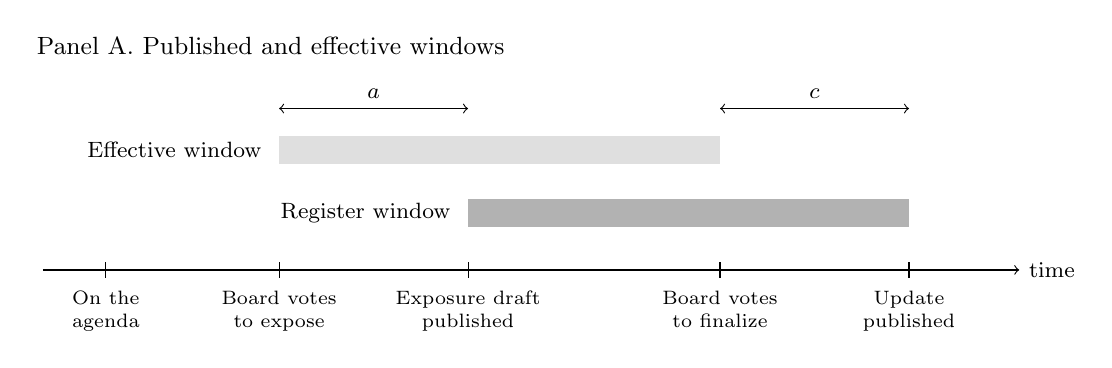
\begin{tikzpicture}[x=1cm,y=1cm,font=\footnotesize]
  \node[anchor=west,font=\small] at (-0.2,2.85) {Panel A. Published and effective windows};
  \draw[->] (0,0) -- (12.4,0) node[right] {time};
  \foreach \x/\lab in {0.8/{On the\\agenda}, 3.0/{Board votes\\to expose}, 5.4/{Exposure draft\\published}, 8.6/{Board votes\\to finalize}, 11.0/{Update\\published}}{
    \draw (\x,0.1) -- (\x,-0.1);
    \node[below,align=center,font=\scriptsize] at (\x,-0.15) {\lab};
  }
  \fill[gray!60] (5.4,0.55) rectangle (11.0,0.9);
  \node[left] at (5.3,0.725) {Register window};
  \fill[gray!25] (3.0,1.35) rectangle (8.6,1.7);
  \node[left] at (2.9,1.525) {Effective window};
  \draw[<->] (3.0,2.05) -- node[above] {$a$} (5.4,2.05);
  \draw[<->] (8.6,2.05) -- node[above] {$c$} (11.0,2.05);
\end{tikzpicture}

\vspace{1.5em}

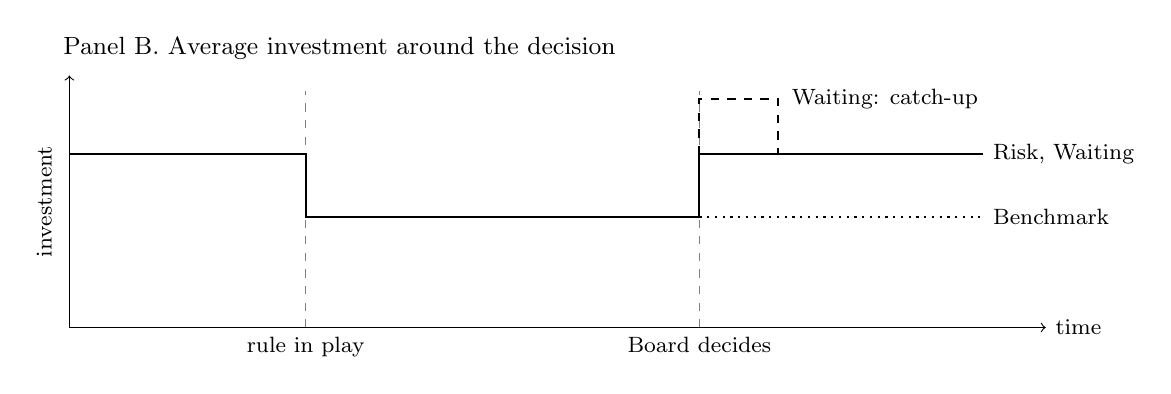
\begin{tikzpicture}[x=1cm,y=1cm,font=\footnotesize]
  \node[anchor=west,font=\small] at (-0.2,3.55) {Panel B. Average investment around the decision};
  \draw[->] (0,0) -- (12.4,0) node[right] {time};
  \draw[->] (0,0) -- (0,3.2);
  \node[rotate=90,anchor=south] at (-0.1,1.6) {investment};
  \draw[gray,dashed] (3,0) -- (3,3.0);
  \draw[gray,dashed] (8,0) -- (8,3.0);
  \node[below] at (3,0) {rule in play};
  \node[below] at (8,0) {Board decides};
  \draw[thick] (0,2.2) -- (3,2.2) -- (3,1.4) -- (8,1.4);
  \draw[thick,dotted] (8,1.4) -- (11.6,1.4) node[right] {Benchmark};
  \draw[thick] (8,1.4) -- (8,2.2) -- (11.6,2.2) node[right] {Risk, Waiting};
  \draw[thick,dashed] (8,2.2) -- (8,2.9) -- (9,2.9) -- (9,2.2);
  \node[right] at (9.05,2.9) {Waiting: catch-up};
\end{tikzpicture}
\caption{Pending Rules in the Model}\label{fig:model}
\par\medskip
\begin{minipage}{\linewidth}\footnotesize
\emph{Notes:} Panel A illustrates Proposition~\ref{prop:model:timing}. The register dates a proposal from the publication of its exposure draft to the publication of the final Update. In the model, the rule is effectively pending from the Board's decision to expose it to its decision to finalize it, which precede publication by $a$ and $c$ quarters. Panel B illustrates Propositions~\ref{prop:model:pending} and~\ref{prop:model:decision}. In the benchmark, investment falls only if the proposal is expected to worsen the reading, and on average it stays at the lower level once the Board decides. In both variants, the proposal leaves the expected reading unchanged; investment falls while the rule is pending and recovers when the Board decides, and in the waiting variant the postponed projects are undertaken at the decision. The pending level is drawn equal in the three cases for comparison.
\end{minipage}
\end{figure}

% ---------------------------------------------------------------------
\subsection{How the Manager Holds Back}\label{sec:model:holdback}

\begin{proposition}[Risk or waiting]\label{prop:model:holdback}
\leavevmode
\begin{enumerate}[label=(\roman*)]
  \item \emph{Investment opportunities.} In the risk variant, $\partial^{2}I_R/\partial\sigma^{2}\partial\gamma<0$ and $\partial^{2}\ln I_R/\partial\sigma^{2}\partial\gamma=0$. In the waiting variant, $\partial^{2}\ln I_W/\partial\sigma^{2}\partial\gamma>0$, and $\partial^{2}I_W/\partial\sigma^{2}\partial\gamma>0$ whenever fewer than a quarter of the projects are postponed.
  \item \emph{Irreversibility.} Suppose investment made while a proposal is pending can be adjusted after the decision at cost $\tfrac{k}{2}(\Delta I)^{2}$, and that $\theta$ is distributed symmetrically around $\bar\theta$. In the waiting variant, the share of projects postponed is $\lambda^{2}\sigma^{2}k/[(1+k)(A^{2}+\lambda^{2}\sigma^{2})]$, which increases in $k$. In the risk variant, the decline in investment is $Ax(1+k)/[1+k(1+x)]$ with $x\equiv\rho\lambda^{2}\sigma^{2}$; it equals $Ax$ up to terms of order $x^{2}$ for every $k$ and decreases slightly in $k$. Under the benchmark, investment is $A$ for every $k$.
  \item \emph{Catch-up.} In the waiting variant, postponed investment is undertaken when the Board decides. In the risk variant, there is none to undertake.
\end{enumerate}
\end{proposition}

Part~(i) holds because, in the waiting variant, a project with a high return loses more by waiting and is therefore less likely to be postponed. In the risk variant, the cost of uncertainty rises with the scale of investment, so firms with better opportunities cut more in levels and the same in proportion. Part~(ii) extends the familiar result that irreversibility raises the value of waiting \citep{dixit1994investment}. It holds in the waiting variant but not, to first order, in the risk variant. There, the ability to adjust after the decision makes the initial investment matter less in two ways at once, for expected value and for the exposure to the reading, and the two effects cancel to first order.

The evidence on these interactions was gathered to test other channels, but read through Proposition~\ref{prop:model:holdback} it favors waiting. The interaction of Pipeline Exposure with Tobin's $q$ in Table~\ref{tab:learning} is positive: 0.581 ($t=1.44$) for the investment rate and 0.651 ($t=2.12$) for total investment. The risk variant predicts a negative interaction in levels. The interaction with asset redeployability in Table~\ref{tab:realoptions} is also positive, 0.413 ($t=1.70$), as the waiting variant predicts and neither the risk variant nor the benchmark does, although it is not significant without oil and gas firms. % memo v7
The result that seems to point the other way is the absence of catch-up in the quarters after a standard is finalized. The catch-up test in Table~\ref{tab:realoptions}, however, begins in the quarter after the resolution quarter. The waiting variant predicts that postponed investment is undertaken as soon as the Board decides, which by Proposition~\ref{prop:model:timing} is typically before the Update is published. The catch-up would then fall in the resolution quarter or earlier, and part of it would be in the Resolving coefficient itself.

% ---------------------------------------------------------------------
\subsection{The Model and the Evidence}\label{sec:model:evidence}

Table~\ref{tab:model:evidence} sets the predictions of the benchmark and the two variants against the evidence. Three conclusions follow. First, the recovery when proposals are resolved rules out the anticipation benchmark and, with it, the view that firms simply price in what proposals are expected to require. Second, the ownership gradient locates the channel in how reported amounts are read rather than in cash flows. A pending rule could also lower investment because it changes the cash-flow payoff of irreversible investment, for example through compliance costs, or because preparing for it absorbs resources. Neither effect would depend on who holds the stock, and the second would persist after a standard is finalized. Third, between the two ways of holding back, the evidence favors waiting, provided that postponed investment returns when the Board decides. The results on the cost of capital and on price informativeness do not distinguish the benchmark from the two variants. They are the reason the model has no investor risk premia and no managerial learning from prices.

\begin{table}[tbp]
\centering
\caption{Predictions and Evidence}\label{tab:model:evidence}
\medskip
\small
\begin{tabular}{@{}lllccc@{}}
\toprule
 & & & \multicolumn{3}{c}{Prediction}\\
\cmidrule(l){4-6}
 & Estimate & Table & Benchmark & Risk & Waiting\\
\midrule
Investment while pending & $-1.531$ & \ref{tab:investment} & $-$\rlap{$^{a}$} & $-$ & $-$\\
Recovery at resolution (offset) & 0.88, 0.90 & \ref{tab:timing} & $0$ & $+$ & $+$\rlap{$^{b}$}\\
\addlinespace
\emph{Interaction with}\\
\quad transient (dedicated) ownership & $-1.012$ ($+0.609$) & \ref{tab:ownership} & $-$ ($+$)\rlap{$^{c}$} & $-$ ($+$) & $-$ ($+$)\\
\quad Tobin's $q$ & $+0.581$, $+0.651$ & \ref{tab:learning} & $0$ & $-$ & $+$\\
\quad asset redeployability & $+0.413$ & \ref{tab:realoptions} & $0$ & $0$ & $+$\\
\addlinespace
Catch-up after the resolution quarter & n.s. & \ref{tab:realoptions} & $0$ & $0$ & $0$\rlap{$^{d}$}\\
\bottomrule
\end{tabular}
% Estimates: memo v7.
\par\medskip
\begin{minipage}{\linewidth}\footnotesize
\emph{Notes:} Estimates are from the tables listed and are per standard deviation of Pipeline Exposure, multiplied by 1,000. The offset is the Resolving coefficient divided by minus the Active coefficient, in the resolution quarter and in the next. The two estimates for Tobin's $q$ are for the investment rate ($t=1.44$) and for total investment ($t=2.12$). The redeployability estimate has $t=1.70$ and is not significant without oil and gas firms. Predictions: Benchmark, Lemma~\ref{lem:model:benchmark}; Risk and Waiting, the two variants of Section~\ref{sec:model:setup}; the signs for Tobin's $q$ are for the level of investment. $^{a}$If proposals are expected to worsen the reading ($\bar\theta<\theta_0$). $^{b}$Including the catch-up of postponed projects when the Board decides (Proposition~\ref{prop:model:decision}). $^{c}$If the expected content of proposals affects investment through the reading. $^{d}$If postponed investment is undertaken when the Board decides, which Proposition~\ref{prop:model:timing} places in the resolution quarter or earlier; positive if it returns gradually.
\end{minipage}
\end{table}

% ---------------------------------------------------------------------
\subsection{Further Predictions}\label{sec:model:further}

The model makes predictions that the evidence so far does not test. Two of them concern the pipeline itself.

\begin{proposition}[Exposure portfolio]\label{prop:model:portfolio}
Let $e_{i,p,q}\equiv\sum_{o\in O_p}s_{i,o,q}/|O_p|$ be firm $i$'s exposure to proposal $p$, so that $\sum_{p\in P_q}e_{i,p,q}$ is Pipeline Exposure (Equation~\eqref{eq:components}). Suppose proposal $p$ shifts the firm's reading by $e_{i,p,q}\Delta_p$, where the $\Delta_p$ are independent with variances $\sigma_p^{2}$. Then the variance of the firm's reading is
\[
  \sigma_{i,q}^{2}=\sum_{p\in P_q}e_{i,p,q}^{2}\,\sigma_p^{2}.
\]
For a given Pipeline Exposure and equal $\sigma_p^{2}$, $\sigma_{i,q}^{2}$ increases with the concentration of exposure across proposals.
\end{proposition}

Pipeline Exposure is the sum of the weights $e_{i,p,q}$. By Propositions~\ref{prop:model:pending} and~\ref{prop:model:portfolio}, investment responds instead to the sum of their squares, weighted by the uncertainty of each proposal. Two firms with the same Pipeline Exposure should therefore respond differently if one of them has its exposure concentrated in a few proposals.

\begin{proposition}[Contested proposals]\label{prop:model:contested}
Suppose proposal $p$ is finalized with probability $\pi_p$, in which case it shifts the reading by $\Delta_p$, and is otherwise withdrawn. Then $\sigma_p^{2}=\pi_p(1-\pi_p)\Delta_p^{2}$, which is largest at $\pi_p=1/2$. The decline in investment in Proposition~\ref{prop:model:pending} is therefore largest for proposals that the Board could decide either way. Under the benchmark, the effect of the proposal, $\lambda\pi_p\Delta_p$, is monotone in $\pi_p$.
\end{proposition}

\begin{remark}[Expected time to decision]\label{rem:model:hazard}
Suppose a postponed project survives each quarter with probability $\phi_j$, discounting included, and the Board decides with probability $h$ per quarter. Waiting until the decision then retains the fraction $\delta_j=\phi_jh/[1-\phi_j(1-h)]$ of the project's value, which increases in $h$. In the waiting variant, a proposal therefore lowers investment more when a decision is expected soon. In the risk variant, the decline does not depend on $h$.
\end{remark}

These results and the earlier propositions point to seven tests, each with the data it requires.
\begin{itemize}
  \item \emph{Timing} (Proposition~\ref{prop:model:timing}). Date each proposal by the Board meetings at which it voted to expose the proposal and to finalize it, which the minutes record. With these dates, the Entering and Resolving coefficients should match the share of the quarter in which the rule is pending in the risk variant. In the waiting variant, investment should exceed that benchmark in the quarter of the decision.
  \item \emph{Concentration} (Proposition~\ref{prop:model:portfolio}). Add $\sum_p e_{i,p,q}^{2}\sigma_p^{2}$ to the investment regression. The model predicts that it carries the effect of Pipeline Exposure.
  \item \emph{Contestedness} (Proposition~\ref{prop:model:contested}). Code the position of each comment letter on its proposal, and whether the exposure draft carries the alternative views of dissenting Board members. The decline should be largest where support and opposition are balanced.
  \item \emph{Expected time to decision} (Remark~\ref{rem:model:hazard}). Code the stage of deliberation from the minutes. The waiting variant predicts larger declines as a decision approaches.
  \item \emph{Managerial incentives} (Propositions~\ref{prop:model:pending} and~\ref{prop:model:intensity}). Managers with equity that vests soon place more weight on the short-term price \citep{edmans2017equity}, which raises $\lambda$ in both variants. The risk variant adds that the decline should be steeper where managerial wealth is more sensitive to the stock price and flatter where compensation is convex \citep{core2002estimating}.
  \item \emph{Firms without traded equity} ($\lambda=0$). Firms that file a 10-K because of public debt but have no traded equity should show no decline, whereas channels that work through cash flows predict one \citep[compare][]{asker2015corporate}.
  \item \emph{The implementation window.} Between a final Update and its effective date, the rule is decided, so the model predicts no decline. A burden of implementation predicts one.
\end{itemize}

Each test uses data that the model, rather than the reduced-form evidence, identifies as relevant: when the Board decides rather than when it publishes, how contested a proposal is, how concentrated a firm's exposure is, and whether anyone reads the firm's reported amounts.
 after the investment results it explains, and
% % =====================================================================
% model_appendix.tex -- proofs for "A Model of Investment under a Pending Rule"
% Use: \input{model_appendix} inside the appendix. The algebra is checked
% symbolically in PipelineExposure/model_checks.py.
% =====================================================================

\section{Proofs for Section~\ref{sec:model}}\label{app:model}

Throughout, write $z\equiv\theta-\bar\theta$, so that $E[z]=0$ and $E[z^{2}]=\sigma^{2}$, and let
\[
  \Pi(\theta)\equiv\max_{I}\,\bigl[V(I)+\lambda\theta I\bigr]=\tfrac12(\gamma+\lambda\theta)^{2},
\]
attained at $I=\gamma+\lambda\theta$. Since $E[(\gamma+\lambda\theta)^{2}]=A^{2}+\lambda^{2}\sigma^{2}$, $E[\Pi(\theta)]=\tfrac12(A^{2}+\lambda^{2}\sigma^{2})$.

\paragraph{Proof of Lemma~\ref{lem:model:benchmark}.}
(i) With $\rho=0$, the manager maximizes $E[U(I;\theta)]=\gamma I-\tfrac12 I^{2}+\lambda\bar\theta I$, because $\varepsilon$ has mean zero. The objective is strictly concave, and the first-order condition gives $I=\gamma+\lambda\bar\theta=A$, which depends on the distribution of $\theta$ only through $\bar\theta$.

(ii) Once $\theta$ is known, investment is $\gamma+\lambda\theta$, so it changes by $\lambda(\theta-\bar\theta)=\lambda z$, whose expectation is zero.

(iii) Let the firm report $R=a+\theta I+\eta$, where $a\sim N(\bar a,\sigma_a^{2})$ is a component of firm value unrelated to the project and $\eta\sim N(0,\sigma_\eta^{2})$; $a$, $\eta$ and $\theta$ are mutually independent. Investors observe $R$ and the decided $\theta$ but not $a$ or $I$, and they conjecture investment $\hat I$. They set
\[
  P=E\bigl[a+V(I)\mid R,\theta\bigr]=\bar a+\beta\,(R-\bar a-\theta\hat I)+V(\hat I),\qquad
  \beta\equiv\frac{\sigma_a^{2}}{\sigma_a^{2}+\sigma_\eta^{2}},
\]
so that $P=\bar a+\beta(a-\bar a+\eta)+V(\hat I)+\beta\theta(I-\hat I)$. The manager chooses $I$ before $\theta$ is known and maximizes the mean minus $\rho/2$ times the variance of $(1-\omega)[a+V(I)]+\omega P$. The only term that depends on both $I$ and $\theta$ is $\omega\beta\theta(I-\hat I)$. Its variance is $\omega^{2}\beta^{2}\sigma^{2}(I-\hat I)^{2}$, and its covariance with the remaining random terms, which involve only $a$ and $\eta$, is zero. The first-order condition is
\[
  (1-\omega)(\gamma-I)+\omega\beta\bar\theta-\rho\,\omega^{2}\beta^{2}\sigma^{2}\,(I-\hat I)=0,
\]
and the objective is strictly concave in $I$. In equilibrium $I=\hat I$, so the last term vanishes and $\hat I=\gamma+\omega\beta\bar\theta/(1-\omega)$, which does not depend on $\sigma^{2}$. \qed

\paragraph{Proof of Proposition~\ref{prop:model:pending}.}
(i) Because $\varepsilon$ is independent of $\theta$, $\mathrm{Var}[U(I;\theta)]=\lambda^{2}\sigma^{2}I^{2}+\omega^{2}\mathrm{Var}(\varepsilon)$. The manager therefore maximizes $\gamma I-\tfrac12 I^{2}+\lambda\bar\theta I-\tfrac{\rho}{2}\lambda^{2}\sigma^{2}I^{2}$, which is strictly concave, and the first-order condition gives $I_R=A/(1+\rho\lambda^{2}\sigma^{2})$. Then
\[
  \frac{\partial I_R}{\partial\sigma^{2}}=-\frac{A\rho\lambda^{2}}{(1+\rho\lambda^{2}\sigma^{2})^{2}}<0\quad\text{for }\lambda\neq0.
\]

(ii) Undertaking project $j$ now yields $\max_I E[U(I;\theta)]=\tfrac12A^{2}$, by Lemma~\ref{lem:model:benchmark}(i). Postponing it yields $\delta_jE[\Pi(\theta)]=\tfrac12\delta_j(A^{2}+\lambda^{2}\sigma^{2})$. Hence the project is postponed if and only if $\delta_j>\delta^{*}$. Each project undertaken now invests $A$, and with $\delta_j$ uniform a mass $\delta^{*}$ of projects is undertaken, so $I_W=A\delta^{*}$ and
\[
  \frac{\partial I_W}{\partial\sigma^{2}}=-\frac{A^{3}\lambda^{2}}{(A^{2}+\lambda^{2}\sigma^{2})^{2}}<0\quad\text{for }\lambda\neq0.
\]
For a general distribution $G$ of $\delta_j$ with a positive density, $I_W=A\,G(\delta^{*})$, which decreases in $\sigma^{2}$ because $\delta^{*}$ does.

(iii) Set $\lambda=0$ in (i) and (ii). \qed

\paragraph{Proof of Proposition~\ref{prop:model:intensity}.}
(i) $A-I_R=A\rho\lambda^{2}\sigma^{2}/(1+\rho\lambda^{2}\sigma^{2})=A\rho\lambda^{2}\sigma^{2}+O(\sigma^{4})$ and $A-I_W=A\lambda^{2}\sigma^{2}/(A^{2}+\lambda^{2}\sigma^{2})=\lambda^{2}\sigma^{2}/A+O(\sigma^{4})$.

(ii) With $\bar\theta=0$, $A=\gamma$ and
\[
  \frac{\partial^{2}I_R}{\partial\sigma^{2}\partial\lambda}=-\frac{2\gamma\rho\lambda\,(1-\rho\lambda^{2}\sigma^{2})}{(1+\rho\lambda^{2}\sigma^{2})^{3}},\qquad
  \frac{\partial^{2}I_W}{\partial\sigma^{2}\partial\lambda}=-\frac{2\gamma^{3}\lambda\,(\gamma^{2}-\lambda^{2}\sigma^{2})}{(\gamma^{2}+\lambda^{2}\sigma^{2})^{3}}.
\]
For $\lambda>0$, the first is negative if and only if $\rho\lambda^{2}\sigma^{2}<1$, which is equivalent to $I_R>A/2$, and the second is negative if and only if $\lambda^{2}\sigma^{2}<\gamma^{2}$, which is equivalent to $\delta^{*}>1/2$. \qed

\paragraph{Proof of Proposition~\ref{prop:model:decision}.}
Once $\theta$ is known there is no uncertainty about the reading, so in both variants new investment maximizes $V(I)+\lambda\theta I$ and equals $\gamma+\lambda\theta$, whose mean is $A$. (i) The average recovery is therefore $A-I_R$, and no project was postponed. (ii) New investment recovers on average from $A\delta^{*}$ to $A$. Each postponed project is undertaken at the decision, because waiting longer only loses value. This adds a mass $1-\delta^{*}$ of projects, each of mean scale $A$, so investment in the period of the decision is on average $A(2-\delta^{*})>A$. (iii) follows from Lemma~\ref{lem:model:benchmark}(ii). \qed

\paragraph{Proof of Proposition~\ref{prop:model:timing}.}
Let $u\sim U[0,1]$ be the point in its quarter at which a document is published, and let $f$ be the share of a quarter in which the rule is effectively pending, so that investment in the quarter is lowered by $|\beta|f$. A proposal pending throughout the quarter has $f=1$, and each coefficient measures the difference from such a proposal, $|\beta|(1-E[f])$.

In the resolution quarter, the rule is effectively decided at $u-c$ if $u>c$ and in the previous quarter otherwise, so $f=\max\{0,u-c\}$ and
\[
  E[f]=\int_{c}^{1}(u-c)\,du=\tfrac12(1-c)^{2}.
\]
The Resolving coefficient is therefore $|\beta|[1-(1-c)^{2}/2]$. In the following quarter the resolved proposal has $f=0$, so the coefficient is $|\beta|$. In the issue quarter, the rule is effectively pending from $u-a$ if $u>a$ and throughout the quarter otherwise, so $f=1-\max\{0,u-a\}$, $E[f]=1-(1-a)^{2}/2$, and the Entering coefficient is $|\beta|(1-a)^{2}/2$. Setting $a=c=0$ gives (iii). In the waiting variant, the postponed projects are undertaken when the Board decides (Proposition~\ref{prop:model:decision}), which falls in the resolution quarter if $u>c$ and in the quarter before otherwise; this gives (iv).

With the estimates in Table~\ref{tab:timing}, $(1-a)^{2}/2=0.101/1.725$ and $1-(1-c)^{2}/2=1.518/1.725$ give $a=0.66$ and $c=0.51$, or 60 and 46 days at 91 days per quarter. % memo v7
\qed

\paragraph{Proof of Proposition~\ref{prop:model:holdback}.}
(i) Since $\partial A/\partial\gamma=1$, differentiating $\partial I_R/\partial\sigma^{2}=-A\rho\lambda^{2}/(1+\rho\lambda^{2}\sigma^{2})^{2}$ with respect to $\gamma$ gives $-\rho\lambda^{2}/(1+\rho\lambda^{2}\sigma^{2})^{2}<0$, and $\partial\ln I_R/\partial\sigma^{2}=-\rho\lambda^{2}/(1+\rho\lambda^{2}\sigma^{2})$ does not depend on $\gamma$. In the waiting variant, $\partial\ln I_W/\partial\sigma^{2}=-\lambda^{2}/(A^{2}+\lambda^{2}\sigma^{2})$, whose derivative with respect to $\gamma$ is $2A\lambda^{2}/(A^{2}+\lambda^{2}\sigma^{2})^{2}>0$, and
\[
  \frac{\partial^{2}I_W}{\partial\sigma^{2}\partial\gamma}=\frac{\lambda^{2}A^{2}\,(A^{2}-3\lambda^{2}\sigma^{2})}{(A^{2}+\lambda^{2}\sigma^{2})^{3}},
\]
which is positive if and only if $A^{2}>3\lambda^{2}\sigma^{2}$, that is, if and only if $1-\delta^{*}<1/4$.

(ii) Let the manager invest $I_0$ while the proposal is pending and, once $\theta$ is known, choose $I_1$ at adjustment cost $\tfrac{k}{2}(I_1-I_0)^{2}$, with $k>0$. Write $m\equiv\gamma+\lambda\theta=A+\lambda z$. The optimal adjustment is $I_1=(m+kI_0)/(1+k)$, and the resulting payoff is
\[
  \pi(z;I_0)=mI_0-\tfrac12I_0^{2}+\frac{(m-I_0)^{2}}{2(1+k)}.
\]
Hence
\[
  E[\pi]=AI_0-\tfrac12I_0^{2}+\frac{(A-I_0)^{2}+\lambda^{2}\sigma^{2}}{2(1+k)},
\]
which is maximized at $I_0=A$ with value $\tfrac12[A^{2}+\lambda^{2}\sigma^{2}/(1+k)]$. This proves the claim for the benchmark. In the waiting variant, postponing project $j$ still yields $\tfrac12\delta_j(A^{2}+\lambda^{2}\sigma^{2})$, so the project is postponed if and only if
\[
  \delta_j>\frac{A^{2}+\lambda^{2}\sigma^{2}/(1+k)}{A^{2}+\lambda^{2}\sigma^{2}},
\]
and the share postponed is $\lambda^{2}\sigma^{2}k/[(1+k)(A^{2}+\lambda^{2}\sigma^{2})]$. Its derivative with respect to $k$ is $\lambda^{2}\sigma^{2}/[(1+k)^{2}(A^{2}+\lambda^{2}\sigma^{2})]>0$.

In the risk variant, $\pi$ is quadratic in $z$, with linear coefficient $c_1=\lambda(A+kI_0)/(1+k)$ and quadratic coefficient $c_2=\lambda^{2}/[2(1+k)]$. Because $z$ is symmetric, $E[z^{3}]=0$ and $\mathrm{Var}[\pi]=c_1^{2}\sigma^{2}+c_2^{2}\,\mathrm{Var}(z^{2})$, in which only $c_1$ depends on $I_0$. The objective $E[\pi]-\tfrac{\rho}{2}\mathrm{Var}[\pi]$ is strictly concave in $I_0$, and its first-order condition,
\[
  \frac{k}{1+k}(A-I_0)-\rho\sigma^{2}c_1\,\frac{\lambda k}{1+k}=0,
\]
gives $I_0=A(1+k-x)/[1+k(1+x)]$ with $x\equiv\rho\lambda^{2}\sigma^{2}$. Hence
\[
  A-I_0=\frac{Ax(1+k)}{1+k(1+x)}=Ax-\frac{Ax^{2}k}{1+k}+O(x^{3}),\qquad
  \frac{\partial(A-I_0)}{\partial k}=-\frac{Ax^{2}}{[1+k(1+x)]^{2}}<0.
\]

(iii) follows from Proposition~\ref{prop:model:decision}. \qed

\paragraph{Proof of Proposition~\ref{prop:model:portfolio}.}
The shift in the firm's reading is $\sum_{p}e_{i,p,q}\Delta_p$, whose variance is $\sum_{p}e_{i,p,q}^{2}\sigma_p^{2}$ because the $\Delta_p$ are independent. With $\sigma_p^{2}=\sigma^{2}$ for all $p$ and Pipeline Exposure $X_{i,q}\equiv\sum_pe_{i,p,q}$ held fixed, $\sigma_{i,q}^{2}=\sigma^{2}X_{i,q}^{2}H_{i,q}$, where $H_{i,q}\equiv\sum_p(e_{i,p,q}/X_{i,q})^{2}$ is the Herfindahl index of the firm's exposure across proposals. \qed

\paragraph{Proof of Proposition~\ref{prop:model:contested}.}
The shift is $\Delta_p$ with probability $\pi_p$ and zero otherwise. Its variance, $\pi_p(1-\pi_p)\Delta_p^{2}$, is largest at $\pi_p=1/2$, and the decline in Proposition~\ref{prop:model:pending} increases in the variance. Its mean is $\pi_p\Delta_p$, so under the benchmark investment moves by $\lambda(\bar\theta-\theta_0)=\lambda\pi_p\Delta_p$, which is monotone in $\pi_p$. \qed

\paragraph{Proof of Remark~\ref{rem:model:hazard}.}
While the proposal is pending the problem is stationary, so a manager who prefers to wait in one quarter prefers to wait in every later quarter until the Board decides. The value $W_j$ of holding project $j$ then satisfies $W_j=\phi_j\{hE[\Pi(\theta)]+(1-h)W_j\}$, so $W_j=\delta_jE[\Pi(\theta)]$ with $\delta_j=\phi_jh/[1-\phi_j(1-h)]$, and
\[
  \frac{\partial\delta_j}{\partial h}=\frac{\phi_j(1-\phi_j)}{[1-\phi_j(1-h)]^{2}}>0.
\]
The project is postponed if and only if $\delta_j>\delta^{*}$, that is, if and only if $\phi_j>\delta^{*}/[\delta^{*}+h(1-\delta^{*})]$. This threshold decreases in $h$, so for any distribution of $\phi_j$ with a positive density the share of projects postponed increases in $h$. In the risk variant, $I_R$ does not depend on $h$. \qed
 in the appendix. Packages and theorem environments:
% model_preamble.tex. New references: model_refs.bib.
%
% Labels defined elsewhere in the paper (rename to match):
%   sec:investment   the investment application
%   eq:components    Equation (4), the components of Pipeline Exposure
%   tab:investment   main investment result                   (memo v7, slide 9)
%   tab:timing       Active / Resolving / Entering            (memo v7, slide 10)
%   tab:ownership    transient and dedicated ownership        (memo v7, slide 13)
%   fig:transient    PE slope by transient-share quartile     (memo v7, slide 14)
%   tab:costcapital  implied cost of capital                  (memo v7, slide 16)
%   tab:learning     non-synchronicity, PE x q, PE x return   (memo v7, slide 17)
%   tab:realoptions  redeployability and catch-up             (memo v7, slide 18)
%
% Estimates are quoted from memo v7 (24 September 2026) and marked
% "% memo v7". If the tables change, update them, and recompute a and c
% after Proposition 4 with PipelineExposure/model_checks.py (check TM3).
% =====================================================================

\section{A Model of Investment under a Pending Rule}\label{sec:model}

Section~\ref{sec:investment} shows that firms invest less when more of their accounting is under revision. Three further facts describe the pattern. The decline ends when the Board resolves the proposals behind it (Table~\ref{tab:timing}). It is steeper for firms held by transient institutions and flatter for firms held by dedicated ones (Table~\ref{tab:ownership}). And it comes with neither a higher implied cost of capital nor less informative prices (Tables~\ref{tab:costcapital} and~\ref{tab:learning}). A pending proposal changes no cash flow and may never become a rule. This section asks why investment falls while one is pending, and why it falls in this way.

The answer I propose is that a pending proposal that would change how an investment is recognized or measured makes it uncertain how today's investment will show up in the numbers that short-horizon investors read. A manager who weighs those numbers holds investment back until the reading is known.

The model combines two familiar parts. The first is a manager who places weight on the current stock price, which responds to reported numbers \citep{narayanan1985managerial,stein1989efficient,bebchuk1993short}. This is the channel through which accounting measurement has real effects \citep{kanodia2016real}. The second is an investment decision taken under an uncertainty that will be resolved at a later date \citep{bernanke1983irreversibility,mcdonald1986value,dixit1994investment}. What the pipeline adds is that the rule that will measure an investment is itself undecided when the investment is made. In models of the real effects of accounting, the measurement rule is fixed and known to all. The pipeline is the period in which it is not.

I first set out the environment (Section~\ref{sec:model:setup}). A benchmark shows that uncertainty about the rule does not, by itself, lower investment (Section~\ref{sec:model:benchmark}), which tells us what else the explanation needs. I then derive the model's predictions for investment while a proposal is pending, for its path when the Board decides, and for the two ways in which a manager can hold investment back (Sections~\ref{sec:model:pending}--\ref{sec:model:holdback}). Section~\ref{sec:model:evidence} compares these predictions with the evidence, and Section~\ref{sec:model:further} collects the predictions that the evidence so far does not test. Proofs are in Appendix~\ref{app:model}.

% ---------------------------------------------------------------------
\subsection{Setup}\label{sec:model:setup}

A manager chooses the scale $I\ge 0$ of a project with net present value
\begin{equation}\label{eq:model:npv}
  V(I)=\gamma I-\tfrac{1}{2}I^{2},
\end{equation}
where $\gamma>0$ measures the quality of the firm's investment opportunities.

\paragraph{Reading.} The accounting rule that will govern the project maps each unit of investment into the amounts that short-horizon investors use, such as earnings, leverage and book values, with loading $\theta$. I call $\theta$ the \emph{reading} of the investment. The short-term price is
\begin{equation}\label{eq:model:price}
  P=V(I)+b\,\theta I+\varepsilon,\qquad b\ge 0,
\end{equation}
where $\varepsilon$ has mean zero and is independent of $I$ and $\theta$. The parameter $b$ measures how much the short-term price moves with reported amounts beyond their economic content. It is positive when short-horizon investors anchor on reported amounts \citep{bushee2001institutional,hirshleifer2003limited}.

\paragraph{Objective.} Following \citet{stein1989efficient}, the manager maximizes a weighted average of long-run value and the short-term price, $(1-\omega)V+\omega P$ with $\omega\in[0,1)$. By \eqref{eq:model:price}, this is
\begin{equation}\label{eq:model:objective}
  U(I;\theta)=V(I)+\lambda\,\theta I+\omega\varepsilon,\qquad \lambda\equiv\omega b.
\end{equation}
I call $\lambda$ the \emph{reading intensity}. It is zero if the manager places no weight on the short-term price or if that price does not respond to reported amounts.

\paragraph{The pipeline.} When no proposal is pending, the reading equals its current value $\theta_0$. A proposal that would change how the project is recognized or measured makes the reading uncertain until the Board decides: while the proposal is pending, $\theta$ has mean $\bar\theta$ and variance $\sigma^{2}>0$, and once the Board decides, $\theta$ is known. A proposal that changes neither recognition nor measurement leaves $\theta=\theta_0$. The Board decides with probability $h$ per quarter. Let $A\equiv\gamma+\lambda\bar\theta$ denote investment at the expected reading. I assume $A>0$ and $\gamma+\lambda\theta>0$ for every $\theta$ in the support, so that investment is interior.

\paragraph{Holding back.} I consider two ways in which uncertainty about the reading can lower investment while a proposal is pending.
\begin{itemize}
  \item In the \emph{risk variant}, the manager evaluates the reading with mean--variance preferences, with weight $\rho>0$ on the variance. The weight reflects, for example, undiversified managerial wealth or payoffs that depend on meeting earnings benchmarks \citep{graham2005economic}.
  \item In the \emph{waiting variant}, the manager is risk neutral, but each project $j$ can be postponed until the Board decides. Postponing retains a fraction $\delta_j\in(0,1)$ of the project's value, which reflects discounting and the chance that the opportunity disappears. Across projects, $\delta_j$ is uniform on $(0,1)$.\footnote{The uniform distribution gives closed forms. The results on the level of investment in Propositions~\ref{prop:model:pending} and~\ref{prop:model:decision} hold for any distribution of $\delta_j$ with a positive density.}
\end{itemize}

Two features of the setup deserve comment. The first is $b>0$. If investors saw through reported amounts, $b$ would be zero and how an investment is reported would not matter. Lemma~\ref{lem:model:benchmark}(iii) below shows that uncertainty about the reading also drops out when investors are fully rational and use reported amounts only to infer what they cannot observe. The ownership results in Table~\ref{tab:ownership} speak directly to this assumption, because the decline is concentrated where short-horizon investors hold more of the stock. The second is timing. The register records the dates on which the Board published an exposure draft or a final Update. The Board, however, deliberates and votes at public meetings before it publishes either document, so the period in which a rule is effectively in play need not coincide with the published window. Section~\ref{sec:model:decision} returns to this point.

% ---------------------------------------------------------------------
\subsection{A Benchmark: Anticipation Only}\label{sec:model:benchmark}

\begin{lemma}[Anticipation]\label{lem:model:benchmark}
Suppose the manager is risk neutral ($\rho=0$) and projects cannot be postponed.
\begin{enumerate}[label=(\roman*)]
  \item While a proposal is pending, investment is $A=\gamma+\lambda\bar\theta$. It depends on the distribution of the reading only through its mean.
  \item When the Board decides, investment changes by $\lambda(\theta-\bar\theta)$, which is zero on average.
  \item The same holds if investors are fully rational. If they observe the rule once it is decided, do not observe investment, and price the firm's report given the investment they anticipate, uncertainty about $\theta$ does not affect equilibrium investment even when the manager is risk averse.
\end{enumerate}
\end{lemma}

The lemma describes the most natural rational account of the evidence, in which firms anticipate what proposals will require. It predicts that investment falls while a proposal is pending only if the proposal is expected to worsen the reading ($\bar\theta<\theta_0$). It also predicts that investment does not recover, on average, when the Board decides, because a decision is on average neither good nor bad news. Table~\ref{tab:timing} rejects the second prediction. Holding Active exposure fixed, exposure from proposals resolved in the quarter offsets 88 percent of the Active coefficient in that quarter and 90 percent in the next, although 138 of the 152 proposals were finalized. % memo v7
The lemma therefore tells us what the explanation needs. Reported amounts must move the short-term price in levels ($b>0$), and the manager must have a reason to respond to uncertainty about the reading rather than only to its mean. The two variants supply the two standard reasons: a concave payoff, or the option to wait.

% ---------------------------------------------------------------------
\subsection{Pending Uncertainty and Investment}\label{sec:model:pending}

\begin{proposition}[Pending uncertainty lowers investment]\label{prop:model:pending}
\leavevmode
\begin{enumerate}[label=(\roman*)]
  \item In the risk variant, investment while a proposal is pending is
  \[
    I_R=\frac{A}{1+\rho\lambda^{2}\sigma^{2}},
  \]
  which decreases in $\sigma^{2}$.
  \item In the waiting variant, project $j$ is postponed if and only if
  \[
    \delta_j>\delta^{*}\equiv\frac{A^{2}}{A^{2}+\lambda^{2}\sigma^{2}},
  \]
  and investment while a proposal is pending is $I_W=A\,\delta^{*}=A^{3}/(A^{2}+\lambda^{2}\sigma^{2})$, which decreases in $\sigma^{2}$.
  \item In both variants, investment does not depend on $\sigma^{2}$ when $\lambda=0$.
\end{enumerate}
\end{proposition}

The two variants reach the same prediction by different routes. In the risk variant, each unit of investment is a bet on how it will be read, and the manager takes a smaller bet. In the waiting variant, investing now commits the firm to a scale that is right for the average reading but wrong for the reading that will apply, so the manager postpones the projects that lose least from waiting. In both, the effect vanishes when $\lambda=0$. A pending rule matters for investment only through a price, or a payoff, that responds to how the investment is reported.

\begin{proposition}[Reading intensity]\label{prop:model:intensity}
\leavevmode
\begin{enumerate}[label=(\roman*)]
  \item The decline in investment, $A-I$, equals $A\rho\lambda^{2}\sigma^{2}$ in the risk variant and $\lambda^{2}\sigma^{2}/A$ in the waiting variant, up to terms of order $\sigma^{4}$. In both variants it is proportional to $\lambda^{2}$.
  \item Suppose the proposal leaves the expected reading unchanged, and normalize $\bar\theta=\theta_0=0$. The slope $\partial I/\partial\sigma^{2}$ is steeper for larger $\lambda$ if $\rho\lambda^{2}\sigma^{2}<1$ in the risk variant, that is, if investment falls by less than half, and if $\lambda^{2}\sigma^{2}<\gamma^{2}$ in the waiting variant, that is, if fewer than half of the projects are postponed.
\end{enumerate}
\end{proposition}

Transient institutions raise both components of $\lambda$. They put pressure on managers to deliver near-term results \citep{bushee1998influence}, which raises $\omega$, and the prices of the stocks they hold weight near-term earnings more heavily \citep{bushee2001institutional}, which raises $b$. Dedicated institutions do the opposite. Proposition~\ref{prop:model:intensity} therefore predicts that the investment decline is steeper where transient ownership is higher and flatter where dedicated ownership is higher, which is the pattern in Table~\ref{tab:ownership}. It also predicts a shape. The decline scales with $\lambda^{2}$, whereas under the benchmark of Lemma~\ref{lem:model:benchmark} the effect of a proposal, $\lambda(\bar\theta-\theta_0)$, scales with $\lambda$. If $\lambda$ is proportional to transient ownership, the decline is therefore quadratic in transient ownership under both variants and linear under the benchmark. The quartile estimates in Figure~\ref{fig:transient}, $-0.79$, $-1.05$, $-2.16$ and $-3.15$, are too imprecise to tell the two shapes apart. % memo v7

% ---------------------------------------------------------------------
\subsection{When the Board Decides}\label{sec:model:decision}

\begin{proposition}[The decision]\label{prop:model:decision}
Once the Board decides, new investment is $\gamma+\lambda\theta$ in both variants.
\begin{enumerate}[label=(\roman*)]
  \item In the risk variant, investment recovers on average by $A-I_R=A\rho\lambda^{2}\sigma^{2}/(1+\rho\lambda^{2}\sigma^{2})>0$. No project was postponed, so there is no catch-up.
  \item In the waiting variant, investment recovers on average by $A-I_W>0$. In addition, the postponed projects, a mass $1-\delta^{*}=\lambda^{2}\sigma^{2}/(A^{2}+\lambda^{2}\sigma^{2})$, are undertaken at once, so investment in the period of the decision exceeds its later level.
  \item Under the benchmark of Lemma~\ref{lem:model:benchmark}, investment does not change on average.
\end{enumerate}
\end{proposition}

Both variants account for the recovery in Table~\ref{tab:timing}. They differ in whether postponed investment comes back, and Panel~B of Figure~\ref{fig:model} draws the three paths. The timing of the estimates carries further information, because the register records when documents were published rather than when the Board made up its mind. The next proposition translates the model into the regression of Table~\ref{tab:timing}, which enters exposure from all pending proposals (Active), from proposals issued in the quarter (Entering), and from proposals resolved in the quarter (Resolving).

\begin{proposition}[Timing]\label{prop:model:timing}
Suppose a proposal lowers investment in a quarter in proportion to the share of the quarter during which its rule is effectively pending, with $|\beta|$ the effect of a full quarter, and that publication dates are uniformly distributed within quarters. Let the rule become effectively pending a fraction $a\in[0,1]$ of a quarter before the exposure draft is published, and be effectively decided a fraction $c\in[0,1]$ of a quarter before the final Update is published. Relative to a proposal that is pending throughout the quarter:
\begin{enumerate}[label=(\roman*)]
  \item the coefficient on Entering in the issue quarter is $|\beta|(1-a)^{2}/2$;
  \item the coefficient on Resolving is $|\beta|\,[1-(1-c)^{2}/2]$ in the resolution quarter and $|\beta|$ in the following quarter;
  \item in particular, if the rule is effectively pending exactly during the published window ($a=c=0$), both coefficients equal $|\beta|/2$ in the quarter of publication;
  \item in the waiting variant, investment in the quarter in which the Board decides also contains the catch-up of postponed projects.
\end{enumerate}
\end{proposition}

In Table~\ref{tab:timing}, the Entering coefficient in the issue quarter is 6 percent of the size of the Active coefficient, and the Resolving coefficient in the resolution quarter is 88 percent of it, against one half each if the published window were the effective one. % memo v7
Read through Proposition~\ref{prop:model:timing}, the two estimates imply $a\approx 0.66$ and $c\approx 0.51$: the rule is in play about 60 days before the exposure draft appears and is effectively decided about 46 days before the Update is published.\footnote{The Active coefficient is itself slightly attenuated when effective dates precede publication, because the quarter before the resolution quarter is then partly decided. The attenuation is small when proposals are pending for several quarters, and the calculation ignores it.} Panel~A of Figure~\ref{fig:model} illustrates. Magnitudes of this kind are what the Board's procedure produces, since the Board decides to issue an exposure draft, and later to finalize a standard, at public meetings that typically precede publication by weeks. Two caveats apply. The Entering coefficient is imprecise ($t=0.19$), so $a$ is loosely pinned down. And in the waiting variant, part of the offset in the resolution quarter can be catch-up rather than early resolution, in which case $c$ is smaller. In the following quarter the offset is 0.90, close to the full offset that both variants predict. % memo v7

\begin{figure}[tbp]
\centering
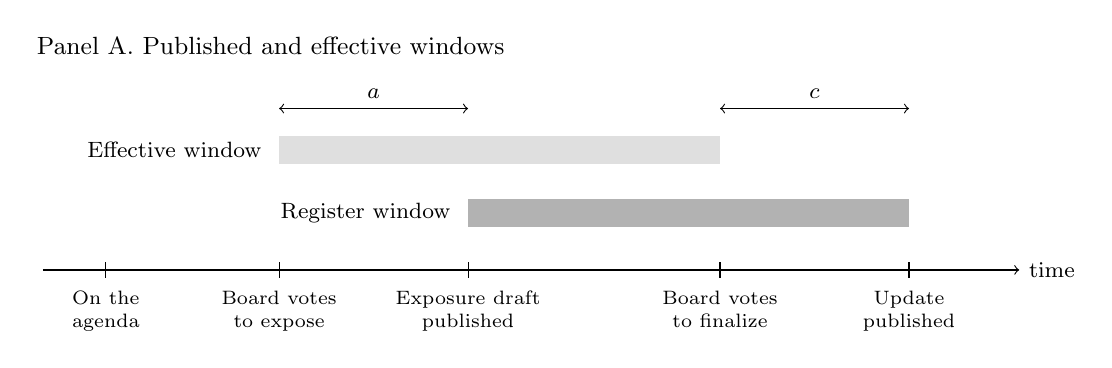
\begin{tikzpicture}[x=1cm,y=1cm,font=\footnotesize]
  \node[anchor=west,font=\small] at (-0.2,2.85) {Panel A. Published and effective windows};
  \draw[->] (0,0) -- (12.4,0) node[right] {time};
  \foreach \x/\lab in {0.8/{On the\\agenda}, 3.0/{Board votes\\to expose}, 5.4/{Exposure draft\\published}, 8.6/{Board votes\\to finalize}, 11.0/{Update\\published}}{
    \draw (\x,0.1) -- (\x,-0.1);
    \node[below,align=center,font=\scriptsize] at (\x,-0.15) {\lab};
  }
  \fill[gray!60] (5.4,0.55) rectangle (11.0,0.9);
  \node[left] at (5.3,0.725) {Register window};
  \fill[gray!25] (3.0,1.35) rectangle (8.6,1.7);
  \node[left] at (2.9,1.525) {Effective window};
  \draw[<->] (3.0,2.05) -- node[above] {$a$} (5.4,2.05);
  \draw[<->] (8.6,2.05) -- node[above] {$c$} (11.0,2.05);
\end{tikzpicture}

\vspace{1.5em}

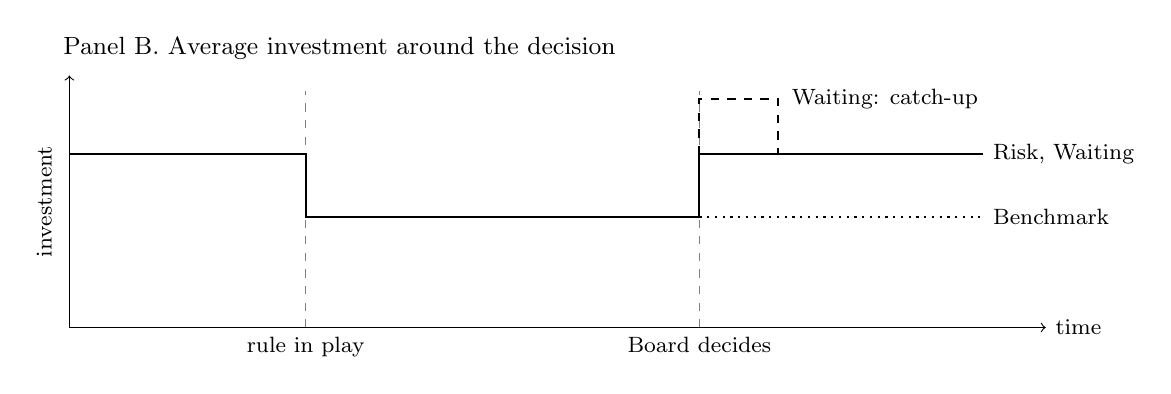
\begin{tikzpicture}[x=1cm,y=1cm,font=\footnotesize]
  \node[anchor=west,font=\small] at (-0.2,3.55) {Panel B. Average investment around the decision};
  \draw[->] (0,0) -- (12.4,0) node[right] {time};
  \draw[->] (0,0) -- (0,3.2);
  \node[rotate=90,anchor=south] at (-0.1,1.6) {investment};
  \draw[gray,dashed] (3,0) -- (3,3.0);
  \draw[gray,dashed] (8,0) -- (8,3.0);
  \node[below] at (3,0) {rule in play};
  \node[below] at (8,0) {Board decides};
  \draw[thick] (0,2.2) -- (3,2.2) -- (3,1.4) -- (8,1.4);
  \draw[thick,dotted] (8,1.4) -- (11.6,1.4) node[right] {Benchmark};
  \draw[thick] (8,1.4) -- (8,2.2) -- (11.6,2.2) node[right] {Risk, Waiting};
  \draw[thick,dashed] (8,2.2) -- (8,2.9) -- (9,2.9) -- (9,2.2);
  \node[right] at (9.05,2.9) {Waiting: catch-up};
\end{tikzpicture}
\caption{Pending Rules in the Model}\label{fig:model}
\par\medskip
\begin{minipage}{\linewidth}\footnotesize
\emph{Notes:} Panel A illustrates Proposition~\ref{prop:model:timing}. The register dates a proposal from the publication of its exposure draft to the publication of the final Update. In the model, the rule is effectively pending from the Board's decision to expose it to its decision to finalize it, which precede publication by $a$ and $c$ quarters. Panel B illustrates Propositions~\ref{prop:model:pending} and~\ref{prop:model:decision}. In the benchmark, investment falls only if the proposal is expected to worsen the reading, and on average it stays at the lower level once the Board decides. In both variants, the proposal leaves the expected reading unchanged; investment falls while the rule is pending and recovers when the Board decides, and in the waiting variant the postponed projects are undertaken at the decision. The pending level is drawn equal in the three cases for comparison.
\end{minipage}
\end{figure}

% ---------------------------------------------------------------------
\subsection{How the Manager Holds Back}\label{sec:model:holdback}

\begin{proposition}[Risk or waiting]\label{prop:model:holdback}
\leavevmode
\begin{enumerate}[label=(\roman*)]
  \item \emph{Investment opportunities.} In the risk variant, $\partial^{2}I_R/\partial\sigma^{2}\partial\gamma<0$ and $\partial^{2}\ln I_R/\partial\sigma^{2}\partial\gamma=0$. In the waiting variant, $\partial^{2}\ln I_W/\partial\sigma^{2}\partial\gamma>0$, and $\partial^{2}I_W/\partial\sigma^{2}\partial\gamma>0$ whenever fewer than a quarter of the projects are postponed.
  \item \emph{Irreversibility.} Suppose investment made while a proposal is pending can be adjusted after the decision at cost $\tfrac{k}{2}(\Delta I)^{2}$, and that $\theta$ is distributed symmetrically around $\bar\theta$. In the waiting variant, the share of projects postponed is $\lambda^{2}\sigma^{2}k/[(1+k)(A^{2}+\lambda^{2}\sigma^{2})]$, which increases in $k$. In the risk variant, the decline in investment is $Ax(1+k)/[1+k(1+x)]$ with $x\equiv\rho\lambda^{2}\sigma^{2}$; it equals $Ax$ up to terms of order $x^{2}$ for every $k$ and decreases slightly in $k$. Under the benchmark, investment is $A$ for every $k$.
  \item \emph{Catch-up.} In the waiting variant, postponed investment is undertaken when the Board decides. In the risk variant, there is none to undertake.
\end{enumerate}
\end{proposition}

Part~(i) holds because, in the waiting variant, a project with a high return loses more by waiting and is therefore less likely to be postponed. In the risk variant, the cost of uncertainty rises with the scale of investment, so firms with better opportunities cut more in levels and the same in proportion. Part~(ii) extends the familiar result that irreversibility raises the value of waiting \citep{dixit1994investment}. It holds in the waiting variant but not, to first order, in the risk variant. There, the ability to adjust after the decision makes the initial investment matter less in two ways at once, for expected value and for the exposure to the reading, and the two effects cancel to first order.

The evidence on these interactions was gathered to test other channels, but read through Proposition~\ref{prop:model:holdback} it favors waiting. The interaction of Pipeline Exposure with Tobin's $q$ in Table~\ref{tab:learning} is positive: 0.581 ($t=1.44$) for the investment rate and 0.651 ($t=2.12$) for total investment. The risk variant predicts a negative interaction in levels. The interaction with asset redeployability in Table~\ref{tab:realoptions} is also positive, 0.413 ($t=1.70$), as the waiting variant predicts and neither the risk variant nor the benchmark does, although it is not significant without oil and gas firms. % memo v7
The result that seems to point the other way is the absence of catch-up in the quarters after a standard is finalized. The catch-up test in Table~\ref{tab:realoptions}, however, begins in the quarter after the resolution quarter. The waiting variant predicts that postponed investment is undertaken as soon as the Board decides, which by Proposition~\ref{prop:model:timing} is typically before the Update is published. The catch-up would then fall in the resolution quarter or earlier, and part of it would be in the Resolving coefficient itself.

% ---------------------------------------------------------------------
\subsection{The Model and the Evidence}\label{sec:model:evidence}

Table~\ref{tab:model:evidence} sets the predictions of the benchmark and the two variants against the evidence. Three conclusions follow. First, the recovery when proposals are resolved rules out the anticipation benchmark and, with it, the view that firms simply price in what proposals are expected to require. Second, the ownership gradient locates the channel in how reported amounts are read rather than in cash flows. A pending rule could also lower investment because it changes the cash-flow payoff of irreversible investment, for example through compliance costs, or because preparing for it absorbs resources. Neither effect would depend on who holds the stock, and the second would persist after a standard is finalized. Third, between the two ways of holding back, the evidence favors waiting, provided that postponed investment returns when the Board decides. The results on the cost of capital and on price informativeness do not distinguish the benchmark from the two variants. They are the reason the model has no investor risk premia and no managerial learning from prices.

\begin{table}[tbp]
\centering
\caption{Predictions and Evidence}\label{tab:model:evidence}
\medskip
\small
\begin{tabular}{@{}lllccc@{}}
\toprule
 & & & \multicolumn{3}{c}{Prediction}\\
\cmidrule(l){4-6}
 & Estimate & Table & Benchmark & Risk & Waiting\\
\midrule
Investment while pending & $-1.531$ & \ref{tab:investment} & $-$\rlap{$^{a}$} & $-$ & $-$\\
Recovery at resolution (offset) & 0.88, 0.90 & \ref{tab:timing} & $0$ & $+$ & $+$\rlap{$^{b}$}\\
\addlinespace
\emph{Interaction with}\\
\quad transient (dedicated) ownership & $-1.012$ ($+0.609$) & \ref{tab:ownership} & $-$ ($+$)\rlap{$^{c}$} & $-$ ($+$) & $-$ ($+$)\\
\quad Tobin's $q$ & $+0.581$, $+0.651$ & \ref{tab:learning} & $0$ & $-$ & $+$\\
\quad asset redeployability & $+0.413$ & \ref{tab:realoptions} & $0$ & $0$ & $+$\\
\addlinespace
Catch-up after the resolution quarter & n.s. & \ref{tab:realoptions} & $0$ & $0$ & $0$\rlap{$^{d}$}\\
\bottomrule
\end{tabular}
% Estimates: memo v7.
\par\medskip
\begin{minipage}{\linewidth}\footnotesize
\emph{Notes:} Estimates are from the tables listed and are per standard deviation of Pipeline Exposure, multiplied by 1,000. The offset is the Resolving coefficient divided by minus the Active coefficient, in the resolution quarter and in the next. The two estimates for Tobin's $q$ are for the investment rate ($t=1.44$) and for total investment ($t=2.12$). The redeployability estimate has $t=1.70$ and is not significant without oil and gas firms. Predictions: Benchmark, Lemma~\ref{lem:model:benchmark}; Risk and Waiting, the two variants of Section~\ref{sec:model:setup}; the signs for Tobin's $q$ are for the level of investment. $^{a}$If proposals are expected to worsen the reading ($\bar\theta<\theta_0$). $^{b}$Including the catch-up of postponed projects when the Board decides (Proposition~\ref{prop:model:decision}). $^{c}$If the expected content of proposals affects investment through the reading. $^{d}$If postponed investment is undertaken when the Board decides, which Proposition~\ref{prop:model:timing} places in the resolution quarter or earlier; positive if it returns gradually.
\end{minipage}
\end{table}

% ---------------------------------------------------------------------
\subsection{Further Predictions}\label{sec:model:further}

The model makes predictions that the evidence so far does not test. Two of them concern the pipeline itself.

\begin{proposition}[Exposure portfolio]\label{prop:model:portfolio}
Let $e_{i,p,q}\equiv\sum_{o\in O_p}s_{i,o,q}/|O_p|$ be firm $i$'s exposure to proposal $p$, so that $\sum_{p\in P_q}e_{i,p,q}$ is Pipeline Exposure (Equation~\eqref{eq:components}). Suppose proposal $p$ shifts the firm's reading by $e_{i,p,q}\Delta_p$, where the $\Delta_p$ are independent with variances $\sigma_p^{2}$. Then the variance of the firm's reading is
\[
  \sigma_{i,q}^{2}=\sum_{p\in P_q}e_{i,p,q}^{2}\,\sigma_p^{2}.
\]
For a given Pipeline Exposure and equal $\sigma_p^{2}$, $\sigma_{i,q}^{2}$ increases with the concentration of exposure across proposals.
\end{proposition}

Pipeline Exposure is the sum of the weights $e_{i,p,q}$. By Propositions~\ref{prop:model:pending} and~\ref{prop:model:portfolio}, investment responds instead to the sum of their squares, weighted by the uncertainty of each proposal. Two firms with the same Pipeline Exposure should therefore respond differently if one of them has its exposure concentrated in a few proposals.

\begin{proposition}[Contested proposals]\label{prop:model:contested}
Suppose proposal $p$ is finalized with probability $\pi_p$, in which case it shifts the reading by $\Delta_p$, and is otherwise withdrawn. Then $\sigma_p^{2}=\pi_p(1-\pi_p)\Delta_p^{2}$, which is largest at $\pi_p=1/2$. The decline in investment in Proposition~\ref{prop:model:pending} is therefore largest for proposals that the Board could decide either way. Under the benchmark, the effect of the proposal, $\lambda\pi_p\Delta_p$, is monotone in $\pi_p$.
\end{proposition}

\begin{remark}[Expected time to decision]\label{rem:model:hazard}
Suppose a postponed project survives each quarter with probability $\phi_j$, discounting included, and the Board decides with probability $h$ per quarter. Waiting until the decision then retains the fraction $\delta_j=\phi_jh/[1-\phi_j(1-h)]$ of the project's value, which increases in $h$. In the waiting variant, a proposal therefore lowers investment more when a decision is expected soon. In the risk variant, the decline does not depend on $h$.
\end{remark}

These results and the earlier propositions point to seven tests, each with the data it requires.
\begin{itemize}
  \item \emph{Timing} (Proposition~\ref{prop:model:timing}). Date each proposal by the Board meetings at which it voted to expose the proposal and to finalize it, which the minutes record. With these dates, the Entering and Resolving coefficients should match the share of the quarter in which the rule is pending in the risk variant. In the waiting variant, investment should exceed that benchmark in the quarter of the decision.
  \item \emph{Concentration} (Proposition~\ref{prop:model:portfolio}). Add $\sum_p e_{i,p,q}^{2}\sigma_p^{2}$ to the investment regression. The model predicts that it carries the effect of Pipeline Exposure.
  \item \emph{Contestedness} (Proposition~\ref{prop:model:contested}). Code the position of each comment letter on its proposal, and whether the exposure draft carries the alternative views of dissenting Board members. The decline should be largest where support and opposition are balanced.
  \item \emph{Expected time to decision} (Remark~\ref{rem:model:hazard}). Code the stage of deliberation from the minutes. The waiting variant predicts larger declines as a decision approaches.
  \item \emph{Managerial incentives} (Propositions~\ref{prop:model:pending} and~\ref{prop:model:intensity}). Managers with equity that vests soon place more weight on the short-term price \citep{edmans2017equity}, which raises $\lambda$ in both variants. The risk variant adds that the decline should be steeper where managerial wealth is more sensitive to the stock price and flatter where compensation is convex \citep{core2002estimating}.
  \item \emph{Firms without traded equity} ($\lambda=0$). Firms that file a 10-K because of public debt but have no traded equity should show no decline, whereas channels that work through cash flows predict one \citep[compare][]{asker2015corporate}.
  \item \emph{The implementation window.} Between a final Update and its effective date, the rule is decided, so the model predicts no decline. A burden of implementation predicts one.
\end{itemize}

Each test uses data that the model, rather than the reduced-form evidence, identifies as relevant: when the Board decides rather than when it publishes, how contested a proposal is, how concentrated a firm's exposure is, and whether anyone reads the firm's reported amounts.
 after the investment results it explains, and
% % =====================================================================
% model_appendix.tex -- proofs for "A Model of Investment under a Pending Rule"
% Use: % =====================================================================
% model_appendix.tex -- proofs for "A Model of Investment under a Pending Rule"
% Use: \input{model_appendix} inside the appendix. The algebra is checked
% symbolically in PipelineExposure/model_checks.py.
% =====================================================================

\section{Proofs for Section~\ref{sec:model}}\label{app:model}

Throughout, write $z\equiv\theta-\bar\theta$, so that $E[z]=0$ and $E[z^{2}]=\sigma^{2}$, and let
\[
  \Pi(\theta)\equiv\max_{I}\,\bigl[V(I)+\lambda\theta I\bigr]=\tfrac12(\gamma+\lambda\theta)^{2},
\]
attained at $I=\gamma+\lambda\theta$. Since $E[(\gamma+\lambda\theta)^{2}]=A^{2}+\lambda^{2}\sigma^{2}$, $E[\Pi(\theta)]=\tfrac12(A^{2}+\lambda^{2}\sigma^{2})$.

\paragraph{Proof of Lemma~\ref{lem:model:benchmark}.}
(i) With $\rho=0$, the manager maximizes $E[U(I;\theta)]=\gamma I-\tfrac12 I^{2}+\lambda\bar\theta I$, because $\varepsilon$ has mean zero. The objective is strictly concave, and the first-order condition gives $I=\gamma+\lambda\bar\theta=A$, which depends on the distribution of $\theta$ only through $\bar\theta$.

(ii) Once $\theta$ is known, investment is $\gamma+\lambda\theta$, so it changes by $\lambda(\theta-\bar\theta)=\lambda z$, whose expectation is zero.

(iii) Let the firm report $R=a+\theta I+\eta$, where $a\sim N(\bar a,\sigma_a^{2})$ is a component of firm value unrelated to the project and $\eta\sim N(0,\sigma_\eta^{2})$; $a$, $\eta$ and $\theta$ are mutually independent. Investors observe $R$ and the decided $\theta$ but not $a$ or $I$, and they conjecture investment $\hat I$. They set
\[
  P=E\bigl[a+V(I)\mid R,\theta\bigr]=\bar a+\beta\,(R-\bar a-\theta\hat I)+V(\hat I),\qquad
  \beta\equiv\frac{\sigma_a^{2}}{\sigma_a^{2}+\sigma_\eta^{2}},
\]
so that $P=\bar a+\beta(a-\bar a+\eta)+V(\hat I)+\beta\theta(I-\hat I)$. The manager chooses $I$ before $\theta$ is known and maximizes the mean minus $\rho/2$ times the variance of $(1-\omega)[a+V(I)]+\omega P$. The only term that depends on both $I$ and $\theta$ is $\omega\beta\theta(I-\hat I)$. Its variance is $\omega^{2}\beta^{2}\sigma^{2}(I-\hat I)^{2}$, and its covariance with the remaining random terms, which involve only $a$ and $\eta$, is zero. The first-order condition is
\[
  (1-\omega)(\gamma-I)+\omega\beta\bar\theta-\rho\,\omega^{2}\beta^{2}\sigma^{2}\,(I-\hat I)=0,
\]
and the objective is strictly concave in $I$. In equilibrium $I=\hat I$, so the last term vanishes and $\hat I=\gamma+\omega\beta\bar\theta/(1-\omega)$, which does not depend on $\sigma^{2}$. \qed

\paragraph{Proof of Proposition~\ref{prop:model:pending}.}
(i) Because $\varepsilon$ is independent of $\theta$, $\mathrm{Var}[U(I;\theta)]=\lambda^{2}\sigma^{2}I^{2}+\omega^{2}\mathrm{Var}(\varepsilon)$. The manager therefore maximizes $\gamma I-\tfrac12 I^{2}+\lambda\bar\theta I-\tfrac{\rho}{2}\lambda^{2}\sigma^{2}I^{2}$, which is strictly concave, and the first-order condition gives $I_R=A/(1+\rho\lambda^{2}\sigma^{2})$. Then
\[
  \frac{\partial I_R}{\partial\sigma^{2}}=-\frac{A\rho\lambda^{2}}{(1+\rho\lambda^{2}\sigma^{2})^{2}}<0\quad\text{for }\lambda\neq0.
\]

(ii) Undertaking project $j$ now yields $\max_I E[U(I;\theta)]=\tfrac12A^{2}$, by Lemma~\ref{lem:model:benchmark}(i). Postponing it yields $\delta_jE[\Pi(\theta)]=\tfrac12\delta_j(A^{2}+\lambda^{2}\sigma^{2})$. Hence the project is postponed if and only if $\delta_j>\delta^{*}$. Each project undertaken now invests $A$, and with $\delta_j$ uniform a mass $\delta^{*}$ of projects is undertaken, so $I_W=A\delta^{*}$ and
\[
  \frac{\partial I_W}{\partial\sigma^{2}}=-\frac{A^{3}\lambda^{2}}{(A^{2}+\lambda^{2}\sigma^{2})^{2}}<0\quad\text{for }\lambda\neq0.
\]
For a general distribution $G$ of $\delta_j$ with a positive density, $I_W=A\,G(\delta^{*})$, which decreases in $\sigma^{2}$ because $\delta^{*}$ does.

(iii) Set $\lambda=0$ in (i) and (ii). \qed

\paragraph{Proof of Proposition~\ref{prop:model:intensity}.}
(i) $A-I_R=A\rho\lambda^{2}\sigma^{2}/(1+\rho\lambda^{2}\sigma^{2})=A\rho\lambda^{2}\sigma^{2}+O(\sigma^{4})$ and $A-I_W=A\lambda^{2}\sigma^{2}/(A^{2}+\lambda^{2}\sigma^{2})=\lambda^{2}\sigma^{2}/A+O(\sigma^{4})$.

(ii) With $\bar\theta=0$, $A=\gamma$ and
\[
  \frac{\partial^{2}I_R}{\partial\sigma^{2}\partial\lambda}=-\frac{2\gamma\rho\lambda\,(1-\rho\lambda^{2}\sigma^{2})}{(1+\rho\lambda^{2}\sigma^{2})^{3}},\qquad
  \frac{\partial^{2}I_W}{\partial\sigma^{2}\partial\lambda}=-\frac{2\gamma^{3}\lambda\,(\gamma^{2}-\lambda^{2}\sigma^{2})}{(\gamma^{2}+\lambda^{2}\sigma^{2})^{3}}.
\]
For $\lambda>0$, the first is negative if and only if $\rho\lambda^{2}\sigma^{2}<1$, which is equivalent to $I_R>A/2$, and the second is negative if and only if $\lambda^{2}\sigma^{2}<\gamma^{2}$, which is equivalent to $\delta^{*}>1/2$. \qed

\paragraph{Proof of Proposition~\ref{prop:model:decision}.}
Once $\theta$ is known there is no uncertainty about the reading, so in both variants new investment maximizes $V(I)+\lambda\theta I$ and equals $\gamma+\lambda\theta$, whose mean is $A$. (i) The average recovery is therefore $A-I_R$, and no project was postponed. (ii) New investment recovers on average from $A\delta^{*}$ to $A$. Each postponed project is undertaken at the decision, because waiting longer only loses value. This adds a mass $1-\delta^{*}$ of projects, each of mean scale $A$, so investment in the period of the decision is on average $A(2-\delta^{*})>A$. (iii) follows from Lemma~\ref{lem:model:benchmark}(ii). \qed

\paragraph{Proof of Proposition~\ref{prop:model:timing}.}
Let $u\sim U[0,1]$ be the point in its quarter at which a document is published, and let $f$ be the share of a quarter in which the rule is effectively pending, so that investment in the quarter is lowered by $|\beta|f$. A proposal pending throughout the quarter has $f=1$, and each coefficient measures the difference from such a proposal, $|\beta|(1-E[f])$.

In the resolution quarter, the rule is effectively decided at $u-c$ if $u>c$ and in the previous quarter otherwise, so $f=\max\{0,u-c\}$ and
\[
  E[f]=\int_{c}^{1}(u-c)\,du=\tfrac12(1-c)^{2}.
\]
The Resolving coefficient is therefore $|\beta|[1-(1-c)^{2}/2]$. In the following quarter the resolved proposal has $f=0$, so the coefficient is $|\beta|$. In the issue quarter, the rule is effectively pending from $u-a$ if $u>a$ and throughout the quarter otherwise, so $f=1-\max\{0,u-a\}$, $E[f]=1-(1-a)^{2}/2$, and the Entering coefficient is $|\beta|(1-a)^{2}/2$. Setting $a=c=0$ gives (iii). In the waiting variant, the postponed projects are undertaken when the Board decides (Proposition~\ref{prop:model:decision}), which falls in the resolution quarter if $u>c$ and in the quarter before otherwise; this gives (iv).

With the estimates in Table~\ref{tab:timing}, $(1-a)^{2}/2=0.101/1.725$ and $1-(1-c)^{2}/2=1.518/1.725$ give $a=0.66$ and $c=0.51$, or 60 and 46 days at 91 days per quarter. % memo v7
\qed

\paragraph{Proof of Proposition~\ref{prop:model:holdback}.}
(i) Since $\partial A/\partial\gamma=1$, differentiating $\partial I_R/\partial\sigma^{2}=-A\rho\lambda^{2}/(1+\rho\lambda^{2}\sigma^{2})^{2}$ with respect to $\gamma$ gives $-\rho\lambda^{2}/(1+\rho\lambda^{2}\sigma^{2})^{2}<0$, and $\partial\ln I_R/\partial\sigma^{2}=-\rho\lambda^{2}/(1+\rho\lambda^{2}\sigma^{2})$ does not depend on $\gamma$. In the waiting variant, $\partial\ln I_W/\partial\sigma^{2}=-\lambda^{2}/(A^{2}+\lambda^{2}\sigma^{2})$, whose derivative with respect to $\gamma$ is $2A\lambda^{2}/(A^{2}+\lambda^{2}\sigma^{2})^{2}>0$, and
\[
  \frac{\partial^{2}I_W}{\partial\sigma^{2}\partial\gamma}=\frac{\lambda^{2}A^{2}\,(A^{2}-3\lambda^{2}\sigma^{2})}{(A^{2}+\lambda^{2}\sigma^{2})^{3}},
\]
which is positive if and only if $A^{2}>3\lambda^{2}\sigma^{2}$, that is, if and only if $1-\delta^{*}<1/4$.

(ii) Let the manager invest $I_0$ while the proposal is pending and, once $\theta$ is known, choose $I_1$ at adjustment cost $\tfrac{k}{2}(I_1-I_0)^{2}$, with $k>0$. Write $m\equiv\gamma+\lambda\theta=A+\lambda z$. The optimal adjustment is $I_1=(m+kI_0)/(1+k)$, and the resulting payoff is
\[
  \pi(z;I_0)=mI_0-\tfrac12I_0^{2}+\frac{(m-I_0)^{2}}{2(1+k)}.
\]
Hence
\[
  E[\pi]=AI_0-\tfrac12I_0^{2}+\frac{(A-I_0)^{2}+\lambda^{2}\sigma^{2}}{2(1+k)},
\]
which is maximized at $I_0=A$ with value $\tfrac12[A^{2}+\lambda^{2}\sigma^{2}/(1+k)]$. This proves the claim for the benchmark. In the waiting variant, postponing project $j$ still yields $\tfrac12\delta_j(A^{2}+\lambda^{2}\sigma^{2})$, so the project is postponed if and only if
\[
  \delta_j>\frac{A^{2}+\lambda^{2}\sigma^{2}/(1+k)}{A^{2}+\lambda^{2}\sigma^{2}},
\]
and the share postponed is $\lambda^{2}\sigma^{2}k/[(1+k)(A^{2}+\lambda^{2}\sigma^{2})]$. Its derivative with respect to $k$ is $\lambda^{2}\sigma^{2}/[(1+k)^{2}(A^{2}+\lambda^{2}\sigma^{2})]>0$.

In the risk variant, $\pi$ is quadratic in $z$, with linear coefficient $c_1=\lambda(A+kI_0)/(1+k)$ and quadratic coefficient $c_2=\lambda^{2}/[2(1+k)]$. Because $z$ is symmetric, $E[z^{3}]=0$ and $\mathrm{Var}[\pi]=c_1^{2}\sigma^{2}+c_2^{2}\,\mathrm{Var}(z^{2})$, in which only $c_1$ depends on $I_0$. The objective $E[\pi]-\tfrac{\rho}{2}\mathrm{Var}[\pi]$ is strictly concave in $I_0$, and its first-order condition,
\[
  \frac{k}{1+k}(A-I_0)-\rho\sigma^{2}c_1\,\frac{\lambda k}{1+k}=0,
\]
gives $I_0=A(1+k-x)/[1+k(1+x)]$ with $x\equiv\rho\lambda^{2}\sigma^{2}$. Hence
\[
  A-I_0=\frac{Ax(1+k)}{1+k(1+x)}=Ax-\frac{Ax^{2}k}{1+k}+O(x^{3}),\qquad
  \frac{\partial(A-I_0)}{\partial k}=-\frac{Ax^{2}}{[1+k(1+x)]^{2}}<0.
\]

(iii) follows from Proposition~\ref{prop:model:decision}. \qed

\paragraph{Proof of Proposition~\ref{prop:model:portfolio}.}
The shift in the firm's reading is $\sum_{p}e_{i,p,q}\Delta_p$, whose variance is $\sum_{p}e_{i,p,q}^{2}\sigma_p^{2}$ because the $\Delta_p$ are independent. With $\sigma_p^{2}=\sigma^{2}$ for all $p$ and Pipeline Exposure $X_{i,q}\equiv\sum_pe_{i,p,q}$ held fixed, $\sigma_{i,q}^{2}=\sigma^{2}X_{i,q}^{2}H_{i,q}$, where $H_{i,q}\equiv\sum_p(e_{i,p,q}/X_{i,q})^{2}$ is the Herfindahl index of the firm's exposure across proposals. \qed

\paragraph{Proof of Proposition~\ref{prop:model:contested}.}
The shift is $\Delta_p$ with probability $\pi_p$ and zero otherwise. Its variance, $\pi_p(1-\pi_p)\Delta_p^{2}$, is largest at $\pi_p=1/2$, and the decline in Proposition~\ref{prop:model:pending} increases in the variance. Its mean is $\pi_p\Delta_p$, so under the benchmark investment moves by $\lambda(\bar\theta-\theta_0)=\lambda\pi_p\Delta_p$, which is monotone in $\pi_p$. \qed

\paragraph{Proof of Remark~\ref{rem:model:hazard}.}
While the proposal is pending the problem is stationary, so a manager who prefers to wait in one quarter prefers to wait in every later quarter until the Board decides. The value $W_j$ of holding project $j$ then satisfies $W_j=\phi_j\{hE[\Pi(\theta)]+(1-h)W_j\}$, so $W_j=\delta_jE[\Pi(\theta)]$ with $\delta_j=\phi_jh/[1-\phi_j(1-h)]$, and
\[
  \frac{\partial\delta_j}{\partial h}=\frac{\phi_j(1-\phi_j)}{[1-\phi_j(1-h)]^{2}}>0.
\]
The project is postponed if and only if $\delta_j>\delta^{*}$, that is, if and only if $\phi_j>\delta^{*}/[\delta^{*}+h(1-\delta^{*})]$. This threshold decreases in $h$, so for any distribution of $\phi_j$ with a positive density the share of projects postponed increases in $h$. In the risk variant, $I_R$ does not depend on $h$. \qed
 inside the appendix. The algebra is checked
% symbolically in PipelineExposure/model_checks.py.
% =====================================================================

\section{Proofs for Section~\ref{sec:model}}\label{app:model}

Throughout, write $z\equiv\theta-\bar\theta$, so that $E[z]=0$ and $E[z^{2}]=\sigma^{2}$, and let
\[
  \Pi(\theta)\equiv\max_{I}\,\bigl[V(I)+\lambda\theta I\bigr]=\tfrac12(\gamma+\lambda\theta)^{2},
\]
attained at $I=\gamma+\lambda\theta$. Since $E[(\gamma+\lambda\theta)^{2}]=A^{2}+\lambda^{2}\sigma^{2}$, $E[\Pi(\theta)]=\tfrac12(A^{2}+\lambda^{2}\sigma^{2})$.

\paragraph{Proof of Lemma~\ref{lem:model:benchmark}.}
(i) With $\rho=0$, the manager maximizes $E[U(I;\theta)]=\gamma I-\tfrac12 I^{2}+\lambda\bar\theta I$, because $\varepsilon$ has mean zero. The objective is strictly concave, and the first-order condition gives $I=\gamma+\lambda\bar\theta=A$, which depends on the distribution of $\theta$ only through $\bar\theta$.

(ii) Once $\theta$ is known, investment is $\gamma+\lambda\theta$, so it changes by $\lambda(\theta-\bar\theta)=\lambda z$, whose expectation is zero.

(iii) Let the firm report $R=a+\theta I+\eta$, where $a\sim N(\bar a,\sigma_a^{2})$ is a component of firm value unrelated to the project and $\eta\sim N(0,\sigma_\eta^{2})$; $a$, $\eta$ and $\theta$ are mutually independent. Investors observe $R$ and the decided $\theta$ but not $a$ or $I$, and they conjecture investment $\hat I$. They set
\[
  P=E\bigl[a+V(I)\mid R,\theta\bigr]=\bar a+\beta\,(R-\bar a-\theta\hat I)+V(\hat I),\qquad
  \beta\equiv\frac{\sigma_a^{2}}{\sigma_a^{2}+\sigma_\eta^{2}},
\]
so that $P=\bar a+\beta(a-\bar a+\eta)+V(\hat I)+\beta\theta(I-\hat I)$. The manager chooses $I$ before $\theta$ is known and maximizes the mean minus $\rho/2$ times the variance of $(1-\omega)[a+V(I)]+\omega P$. The only term that depends on both $I$ and $\theta$ is $\omega\beta\theta(I-\hat I)$. Its variance is $\omega^{2}\beta^{2}\sigma^{2}(I-\hat I)^{2}$, and its covariance with the remaining random terms, which involve only $a$ and $\eta$, is zero. The first-order condition is
\[
  (1-\omega)(\gamma-I)+\omega\beta\bar\theta-\rho\,\omega^{2}\beta^{2}\sigma^{2}\,(I-\hat I)=0,
\]
and the objective is strictly concave in $I$. In equilibrium $I=\hat I$, so the last term vanishes and $\hat I=\gamma+\omega\beta\bar\theta/(1-\omega)$, which does not depend on $\sigma^{2}$. \qed

\paragraph{Proof of Proposition~\ref{prop:model:pending}.}
(i) Because $\varepsilon$ is independent of $\theta$, $\mathrm{Var}[U(I;\theta)]=\lambda^{2}\sigma^{2}I^{2}+\omega^{2}\mathrm{Var}(\varepsilon)$. The manager therefore maximizes $\gamma I-\tfrac12 I^{2}+\lambda\bar\theta I-\tfrac{\rho}{2}\lambda^{2}\sigma^{2}I^{2}$, which is strictly concave, and the first-order condition gives $I_R=A/(1+\rho\lambda^{2}\sigma^{2})$. Then
\[
  \frac{\partial I_R}{\partial\sigma^{2}}=-\frac{A\rho\lambda^{2}}{(1+\rho\lambda^{2}\sigma^{2})^{2}}<0\quad\text{for }\lambda\neq0.
\]

(ii) Undertaking project $j$ now yields $\max_I E[U(I;\theta)]=\tfrac12A^{2}$, by Lemma~\ref{lem:model:benchmark}(i). Postponing it yields $\delta_jE[\Pi(\theta)]=\tfrac12\delta_j(A^{2}+\lambda^{2}\sigma^{2})$. Hence the project is postponed if and only if $\delta_j>\delta^{*}$. Each project undertaken now invests $A$, and with $\delta_j$ uniform a mass $\delta^{*}$ of projects is undertaken, so $I_W=A\delta^{*}$ and
\[
  \frac{\partial I_W}{\partial\sigma^{2}}=-\frac{A^{3}\lambda^{2}}{(A^{2}+\lambda^{2}\sigma^{2})^{2}}<0\quad\text{for }\lambda\neq0.
\]
For a general distribution $G$ of $\delta_j$ with a positive density, $I_W=A\,G(\delta^{*})$, which decreases in $\sigma^{2}$ because $\delta^{*}$ does.

(iii) Set $\lambda=0$ in (i) and (ii). \qed

\paragraph{Proof of Proposition~\ref{prop:model:intensity}.}
(i) $A-I_R=A\rho\lambda^{2}\sigma^{2}/(1+\rho\lambda^{2}\sigma^{2})=A\rho\lambda^{2}\sigma^{2}+O(\sigma^{4})$ and $A-I_W=A\lambda^{2}\sigma^{2}/(A^{2}+\lambda^{2}\sigma^{2})=\lambda^{2}\sigma^{2}/A+O(\sigma^{4})$.

(ii) With $\bar\theta=0$, $A=\gamma$ and
\[
  \frac{\partial^{2}I_R}{\partial\sigma^{2}\partial\lambda}=-\frac{2\gamma\rho\lambda\,(1-\rho\lambda^{2}\sigma^{2})}{(1+\rho\lambda^{2}\sigma^{2})^{3}},\qquad
  \frac{\partial^{2}I_W}{\partial\sigma^{2}\partial\lambda}=-\frac{2\gamma^{3}\lambda\,(\gamma^{2}-\lambda^{2}\sigma^{2})}{(\gamma^{2}+\lambda^{2}\sigma^{2})^{3}}.
\]
For $\lambda>0$, the first is negative if and only if $\rho\lambda^{2}\sigma^{2}<1$, which is equivalent to $I_R>A/2$, and the second is negative if and only if $\lambda^{2}\sigma^{2}<\gamma^{2}$, which is equivalent to $\delta^{*}>1/2$. \qed

\paragraph{Proof of Proposition~\ref{prop:model:decision}.}
Once $\theta$ is known there is no uncertainty about the reading, so in both variants new investment maximizes $V(I)+\lambda\theta I$ and equals $\gamma+\lambda\theta$, whose mean is $A$. (i) The average recovery is therefore $A-I_R$, and no project was postponed. (ii) New investment recovers on average from $A\delta^{*}$ to $A$. Each postponed project is undertaken at the decision, because waiting longer only loses value. This adds a mass $1-\delta^{*}$ of projects, each of mean scale $A$, so investment in the period of the decision is on average $A(2-\delta^{*})>A$. (iii) follows from Lemma~\ref{lem:model:benchmark}(ii). \qed

\paragraph{Proof of Proposition~\ref{prop:model:timing}.}
Let $u\sim U[0,1]$ be the point in its quarter at which a document is published, and let $f$ be the share of a quarter in which the rule is effectively pending, so that investment in the quarter is lowered by $|\beta|f$. A proposal pending throughout the quarter has $f=1$, and each coefficient measures the difference from such a proposal, $|\beta|(1-E[f])$.

In the resolution quarter, the rule is effectively decided at $u-c$ if $u>c$ and in the previous quarter otherwise, so $f=\max\{0,u-c\}$ and
\[
  E[f]=\int_{c}^{1}(u-c)\,du=\tfrac12(1-c)^{2}.
\]
The Resolving coefficient is therefore $|\beta|[1-(1-c)^{2}/2]$. In the following quarter the resolved proposal has $f=0$, so the coefficient is $|\beta|$. In the issue quarter, the rule is effectively pending from $u-a$ if $u>a$ and throughout the quarter otherwise, so $f=1-\max\{0,u-a\}$, $E[f]=1-(1-a)^{2}/2$, and the Entering coefficient is $|\beta|(1-a)^{2}/2$. Setting $a=c=0$ gives (iii). In the waiting variant, the postponed projects are undertaken when the Board decides (Proposition~\ref{prop:model:decision}), which falls in the resolution quarter if $u>c$ and in the quarter before otherwise; this gives (iv).

With the estimates in Table~\ref{tab:timing}, $(1-a)^{2}/2=0.101/1.725$ and $1-(1-c)^{2}/2=1.518/1.725$ give $a=0.66$ and $c=0.51$, or 60 and 46 days at 91 days per quarter. % memo v7
\qed

\paragraph{Proof of Proposition~\ref{prop:model:holdback}.}
(i) Since $\partial A/\partial\gamma=1$, differentiating $\partial I_R/\partial\sigma^{2}=-A\rho\lambda^{2}/(1+\rho\lambda^{2}\sigma^{2})^{2}$ with respect to $\gamma$ gives $-\rho\lambda^{2}/(1+\rho\lambda^{2}\sigma^{2})^{2}<0$, and $\partial\ln I_R/\partial\sigma^{2}=-\rho\lambda^{2}/(1+\rho\lambda^{2}\sigma^{2})$ does not depend on $\gamma$. In the waiting variant, $\partial\ln I_W/\partial\sigma^{2}=-\lambda^{2}/(A^{2}+\lambda^{2}\sigma^{2})$, whose derivative with respect to $\gamma$ is $2A\lambda^{2}/(A^{2}+\lambda^{2}\sigma^{2})^{2}>0$, and
\[
  \frac{\partial^{2}I_W}{\partial\sigma^{2}\partial\gamma}=\frac{\lambda^{2}A^{2}\,(A^{2}-3\lambda^{2}\sigma^{2})}{(A^{2}+\lambda^{2}\sigma^{2})^{3}},
\]
which is positive if and only if $A^{2}>3\lambda^{2}\sigma^{2}$, that is, if and only if $1-\delta^{*}<1/4$.

(ii) Let the manager invest $I_0$ while the proposal is pending and, once $\theta$ is known, choose $I_1$ at adjustment cost $\tfrac{k}{2}(I_1-I_0)^{2}$, with $k>0$. Write $m\equiv\gamma+\lambda\theta=A+\lambda z$. The optimal adjustment is $I_1=(m+kI_0)/(1+k)$, and the resulting payoff is
\[
  \pi(z;I_0)=mI_0-\tfrac12I_0^{2}+\frac{(m-I_0)^{2}}{2(1+k)}.
\]
Hence
\[
  E[\pi]=AI_0-\tfrac12I_0^{2}+\frac{(A-I_0)^{2}+\lambda^{2}\sigma^{2}}{2(1+k)},
\]
which is maximized at $I_0=A$ with value $\tfrac12[A^{2}+\lambda^{2}\sigma^{2}/(1+k)]$. This proves the claim for the benchmark. In the waiting variant, postponing project $j$ still yields $\tfrac12\delta_j(A^{2}+\lambda^{2}\sigma^{2})$, so the project is postponed if and only if
\[
  \delta_j>\frac{A^{2}+\lambda^{2}\sigma^{2}/(1+k)}{A^{2}+\lambda^{2}\sigma^{2}},
\]
and the share postponed is $\lambda^{2}\sigma^{2}k/[(1+k)(A^{2}+\lambda^{2}\sigma^{2})]$. Its derivative with respect to $k$ is $\lambda^{2}\sigma^{2}/[(1+k)^{2}(A^{2}+\lambda^{2}\sigma^{2})]>0$.

In the risk variant, $\pi$ is quadratic in $z$, with linear coefficient $c_1=\lambda(A+kI_0)/(1+k)$ and quadratic coefficient $c_2=\lambda^{2}/[2(1+k)]$. Because $z$ is symmetric, $E[z^{3}]=0$ and $\mathrm{Var}[\pi]=c_1^{2}\sigma^{2}+c_2^{2}\,\mathrm{Var}(z^{2})$, in which only $c_1$ depends on $I_0$. The objective $E[\pi]-\tfrac{\rho}{2}\mathrm{Var}[\pi]$ is strictly concave in $I_0$, and its first-order condition,
\[
  \frac{k}{1+k}(A-I_0)-\rho\sigma^{2}c_1\,\frac{\lambda k}{1+k}=0,
\]
gives $I_0=A(1+k-x)/[1+k(1+x)]$ with $x\equiv\rho\lambda^{2}\sigma^{2}$. Hence
\[
  A-I_0=\frac{Ax(1+k)}{1+k(1+x)}=Ax-\frac{Ax^{2}k}{1+k}+O(x^{3}),\qquad
  \frac{\partial(A-I_0)}{\partial k}=-\frac{Ax^{2}}{[1+k(1+x)]^{2}}<0.
\]

(iii) follows from Proposition~\ref{prop:model:decision}. \qed

\paragraph{Proof of Proposition~\ref{prop:model:portfolio}.}
The shift in the firm's reading is $\sum_{p}e_{i,p,q}\Delta_p$, whose variance is $\sum_{p}e_{i,p,q}^{2}\sigma_p^{2}$ because the $\Delta_p$ are independent. With $\sigma_p^{2}=\sigma^{2}$ for all $p$ and Pipeline Exposure $X_{i,q}\equiv\sum_pe_{i,p,q}$ held fixed, $\sigma_{i,q}^{2}=\sigma^{2}X_{i,q}^{2}H_{i,q}$, where $H_{i,q}\equiv\sum_p(e_{i,p,q}/X_{i,q})^{2}$ is the Herfindahl index of the firm's exposure across proposals. \qed

\paragraph{Proof of Proposition~\ref{prop:model:contested}.}
The shift is $\Delta_p$ with probability $\pi_p$ and zero otherwise. Its variance, $\pi_p(1-\pi_p)\Delta_p^{2}$, is largest at $\pi_p=1/2$, and the decline in Proposition~\ref{prop:model:pending} increases in the variance. Its mean is $\pi_p\Delta_p$, so under the benchmark investment moves by $\lambda(\bar\theta-\theta_0)=\lambda\pi_p\Delta_p$, which is monotone in $\pi_p$. \qed

\paragraph{Proof of Remark~\ref{rem:model:hazard}.}
While the proposal is pending the problem is stationary, so a manager who prefers to wait in one quarter prefers to wait in every later quarter until the Board decides. The value $W_j$ of holding project $j$ then satisfies $W_j=\phi_j\{hE[\Pi(\theta)]+(1-h)W_j\}$, so $W_j=\delta_jE[\Pi(\theta)]$ with $\delta_j=\phi_jh/[1-\phi_j(1-h)]$, and
\[
  \frac{\partial\delta_j}{\partial h}=\frac{\phi_j(1-\phi_j)}{[1-\phi_j(1-h)]^{2}}>0.
\]
The project is postponed if and only if $\delta_j>\delta^{*}$, that is, if and only if $\phi_j>\delta^{*}/[\delta^{*}+h(1-\delta^{*})]$. This threshold decreases in $h$, so for any distribution of $\phi_j$ with a positive density the share of projects postponed increases in $h$. In the risk variant, $I_R$ does not depend on $h$. \qed
 in the appendix. Packages and theorem environments:
% model_preamble.tex. New references: model_refs.bib.
%
% Labels defined elsewhere in the paper (rename to match):
%   sec:investment   the investment application
%   eq:components    Equation (4), the components of Pipeline Exposure
%   tab:investment   main investment result                   (memo v7, slide 9)
%   tab:timing       Active / Resolving / Entering            (memo v7, slide 10)
%   tab:ownership    transient and dedicated ownership        (memo v7, slide 13)
%   fig:transient    PE slope by transient-share quartile     (memo v7, slide 14)
%   tab:costcapital  implied cost of capital                  (memo v7, slide 16)
%   tab:learning     non-synchronicity, PE x q, PE x return   (memo v7, slide 17)
%   tab:realoptions  redeployability and catch-up             (memo v7, slide 18)
%
% Estimates are quoted from memo v7 (24 September 2026) and marked
% "% memo v7". If the tables change, update them, and recompute a and c
% after Proposition 4 with PipelineExposure/model_checks.py (check TM3).
% =====================================================================

\section{A Model of Investment under a Pending Rule}\label{sec:model}

Section~\ref{sec:investment} shows that firms invest less when more of their accounting is under revision. Three further facts describe the pattern. The decline ends when the Board resolves the proposals behind it (Table~\ref{tab:timing}). It is steeper for firms held by transient institutions and flatter for firms held by dedicated ones (Table~\ref{tab:ownership}). And it comes with neither a higher implied cost of capital nor less informative prices (Tables~\ref{tab:costcapital} and~\ref{tab:learning}). A pending proposal changes no cash flow and may never become a rule. This section asks why investment falls while one is pending, and why it falls in this way.

The answer I propose is that a pending proposal that would change how an investment is recognized or measured makes it uncertain how today's investment will show up in the numbers that short-horizon investors read. A manager who weighs those numbers holds investment back until the reading is known.

The model combines two familiar parts. The first is a manager who places weight on the current stock price, which responds to reported numbers \citep{narayanan1985managerial,stein1989efficient,bebchuk1993short}. This is the channel through which accounting measurement has real effects \citep{kanodia2016real}. The second is an investment decision taken under an uncertainty that will be resolved at a later date \citep{bernanke1983irreversibility,mcdonald1986value,dixit1994investment}. What the pipeline adds is that the rule that will measure an investment is itself undecided when the investment is made. In models of the real effects of accounting, the measurement rule is fixed and known to all. The pipeline is the period in which it is not.

I first set out the environment (Section~\ref{sec:model:setup}). A benchmark shows that uncertainty about the rule does not, by itself, lower investment (Section~\ref{sec:model:benchmark}), which tells us what else the explanation needs. I then derive the model's predictions for investment while a proposal is pending, for its path when the Board decides, and for the two ways in which a manager can hold investment back (Sections~\ref{sec:model:pending}--\ref{sec:model:holdback}). Section~\ref{sec:model:evidence} compares these predictions with the evidence, and Section~\ref{sec:model:further} collects the predictions that the evidence so far does not test. Proofs are in Appendix~\ref{app:model}.

% ---------------------------------------------------------------------
\subsection{Setup}\label{sec:model:setup}

A manager chooses the scale $I\ge 0$ of a project with net present value
\begin{equation}\label{eq:model:npv}
  V(I)=\gamma I-\tfrac{1}{2}I^{2},
\end{equation}
where $\gamma>0$ measures the quality of the firm's investment opportunities.

\paragraph{Reading.} The accounting rule that will govern the project maps each unit of investment into the amounts that short-horizon investors use, such as earnings, leverage and book values, with loading $\theta$. I call $\theta$ the \emph{reading} of the investment. The short-term price is
\begin{equation}\label{eq:model:price}
  P=V(I)+b\,\theta I+\varepsilon,\qquad b\ge 0,
\end{equation}
where $\varepsilon$ has mean zero and is independent of $I$ and $\theta$. The parameter $b$ measures how much the short-term price moves with reported amounts beyond their economic content. It is positive when short-horizon investors anchor on reported amounts \citep{bushee2001institutional,hirshleifer2003limited}.

\paragraph{Objective.} Following \citet{stein1989efficient}, the manager maximizes a weighted average of long-run value and the short-term price, $(1-\omega)V+\omega P$ with $\omega\in[0,1)$. By \eqref{eq:model:price}, this is
\begin{equation}\label{eq:model:objective}
  U(I;\theta)=V(I)+\lambda\,\theta I+\omega\varepsilon,\qquad \lambda\equiv\omega b.
\end{equation}
I call $\lambda$ the \emph{reading intensity}. It is zero if the manager places no weight on the short-term price or if that price does not respond to reported amounts.

\paragraph{The pipeline.} When no proposal is pending, the reading equals its current value $\theta_0$. A proposal that would change how the project is recognized or measured makes the reading uncertain until the Board decides: while the proposal is pending, $\theta$ has mean $\bar\theta$ and variance $\sigma^{2}>0$, and once the Board decides, $\theta$ is known. A proposal that changes neither recognition nor measurement leaves $\theta=\theta_0$. The Board decides with probability $h$ per quarter. Let $A\equiv\gamma+\lambda\bar\theta$ denote investment at the expected reading. I assume $A>0$ and $\gamma+\lambda\theta>0$ for every $\theta$ in the support, so that investment is interior.

\paragraph{Holding back.} I consider two ways in which uncertainty about the reading can lower investment while a proposal is pending.
\begin{itemize}
  \item In the \emph{risk variant}, the manager evaluates the reading with mean--variance preferences, with weight $\rho>0$ on the variance. The weight reflects, for example, undiversified managerial wealth or payoffs that depend on meeting earnings benchmarks \citep{graham2005economic}.
  \item In the \emph{waiting variant}, the manager is risk neutral, but each project $j$ can be postponed until the Board decides. Postponing retains a fraction $\delta_j\in(0,1)$ of the project's value, which reflects discounting and the chance that the opportunity disappears. Across projects, $\delta_j$ is uniform on $(0,1)$.\footnote{The uniform distribution gives closed forms. The results on the level of investment in Propositions~\ref{prop:model:pending} and~\ref{prop:model:decision} hold for any distribution of $\delta_j$ with a positive density.}
\end{itemize}

Two features of the setup deserve comment. The first is $b>0$. If investors saw through reported amounts, $b$ would be zero and how an investment is reported would not matter. Lemma~\ref{lem:model:benchmark}(iii) below shows that uncertainty about the reading also drops out when investors are fully rational and use reported amounts only to infer what they cannot observe. The ownership results in Table~\ref{tab:ownership} speak directly to this assumption, because the decline is concentrated where short-horizon investors hold more of the stock. The second is timing. The register records the dates on which the Board published an exposure draft or a final Update. The Board, however, deliberates and votes at public meetings before it publishes either document, so the period in which a rule is effectively in play need not coincide with the published window. Section~\ref{sec:model:decision} returns to this point.

% ---------------------------------------------------------------------
\subsection{A Benchmark: Anticipation Only}\label{sec:model:benchmark}

\begin{lemma}[Anticipation]\label{lem:model:benchmark}
Suppose the manager is risk neutral ($\rho=0$) and projects cannot be postponed.
\begin{enumerate}[label=(\roman*)]
  \item While a proposal is pending, investment is $A=\gamma+\lambda\bar\theta$. It depends on the distribution of the reading only through its mean.
  \item When the Board decides, investment changes by $\lambda(\theta-\bar\theta)$, which is zero on average.
  \item The same holds if investors are fully rational. If they observe the rule once it is decided, do not observe investment, and price the firm's report given the investment they anticipate, uncertainty about $\theta$ does not affect equilibrium investment even when the manager is risk averse.
\end{enumerate}
\end{lemma}

The lemma describes the most natural rational account of the evidence, in which firms anticipate what proposals will require. It predicts that investment falls while a proposal is pending only if the proposal is expected to worsen the reading ($\bar\theta<\theta_0$). It also predicts that investment does not recover, on average, when the Board decides, because a decision is on average neither good nor bad news. Table~\ref{tab:timing} rejects the second prediction. Holding Active exposure fixed, exposure from proposals resolved in the quarter offsets 88 percent of the Active coefficient in that quarter and 90 percent in the next, although 138 of the 152 proposals were finalized. % memo v7
The lemma therefore tells us what the explanation needs. Reported amounts must move the short-term price in levels ($b>0$), and the manager must have a reason to respond to uncertainty about the reading rather than only to its mean. The two variants supply the two standard reasons: a concave payoff, or the option to wait.

% ---------------------------------------------------------------------
\subsection{Pending Uncertainty and Investment}\label{sec:model:pending}

\begin{proposition}[Pending uncertainty lowers investment]\label{prop:model:pending}
\leavevmode
\begin{enumerate}[label=(\roman*)]
  \item In the risk variant, investment while a proposal is pending is
  \[
    I_R=\frac{A}{1+\rho\lambda^{2}\sigma^{2}},
  \]
  which decreases in $\sigma^{2}$.
  \item In the waiting variant, project $j$ is postponed if and only if
  \[
    \delta_j>\delta^{*}\equiv\frac{A^{2}}{A^{2}+\lambda^{2}\sigma^{2}},
  \]
  and investment while a proposal is pending is $I_W=A\,\delta^{*}=A^{3}/(A^{2}+\lambda^{2}\sigma^{2})$, which decreases in $\sigma^{2}$.
  \item In both variants, investment does not depend on $\sigma^{2}$ when $\lambda=0$.
\end{enumerate}
\end{proposition}

The two variants reach the same prediction by different routes. In the risk variant, each unit of investment is a bet on how it will be read, and the manager takes a smaller bet. In the waiting variant, investing now commits the firm to a scale that is right for the average reading but wrong for the reading that will apply, so the manager postpones the projects that lose least from waiting. In both, the effect vanishes when $\lambda=0$. A pending rule matters for investment only through a price, or a payoff, that responds to how the investment is reported.

\begin{proposition}[Reading intensity]\label{prop:model:intensity}
\leavevmode
\begin{enumerate}[label=(\roman*)]
  \item The decline in investment, $A-I$, equals $A\rho\lambda^{2}\sigma^{2}$ in the risk variant and $\lambda^{2}\sigma^{2}/A$ in the waiting variant, up to terms of order $\sigma^{4}$. In both variants it is proportional to $\lambda^{2}$.
  \item Suppose the proposal leaves the expected reading unchanged, and normalize $\bar\theta=\theta_0=0$. The slope $\partial I/\partial\sigma^{2}$ is steeper for larger $\lambda$ if $\rho\lambda^{2}\sigma^{2}<1$ in the risk variant, that is, if investment falls by less than half, and if $\lambda^{2}\sigma^{2}<\gamma^{2}$ in the waiting variant, that is, if fewer than half of the projects are postponed.
\end{enumerate}
\end{proposition}

Transient institutions raise both components of $\lambda$. They put pressure on managers to deliver near-term results \citep{bushee1998influence}, which raises $\omega$, and the prices of the stocks they hold weight near-term earnings more heavily \citep{bushee2001institutional}, which raises $b$. Dedicated institutions do the opposite. Proposition~\ref{prop:model:intensity} therefore predicts that the investment decline is steeper where transient ownership is higher and flatter where dedicated ownership is higher, which is the pattern in Table~\ref{tab:ownership}. It also predicts a shape. The decline scales with $\lambda^{2}$, whereas under the benchmark of Lemma~\ref{lem:model:benchmark} the effect of a proposal, $\lambda(\bar\theta-\theta_0)$, scales with $\lambda$. If $\lambda$ is proportional to transient ownership, the decline is therefore quadratic in transient ownership under both variants and linear under the benchmark. The quartile estimates in Figure~\ref{fig:transient}, $-0.79$, $-1.05$, $-2.16$ and $-3.15$, are too imprecise to tell the two shapes apart. % memo v7

% ---------------------------------------------------------------------
\subsection{When the Board Decides}\label{sec:model:decision}

\begin{proposition}[The decision]\label{prop:model:decision}
Once the Board decides, new investment is $\gamma+\lambda\theta$ in both variants.
\begin{enumerate}[label=(\roman*)]
  \item In the risk variant, investment recovers on average by $A-I_R=A\rho\lambda^{2}\sigma^{2}/(1+\rho\lambda^{2}\sigma^{2})>0$. No project was postponed, so there is no catch-up.
  \item In the waiting variant, investment recovers on average by $A-I_W>0$. In addition, the postponed projects, a mass $1-\delta^{*}=\lambda^{2}\sigma^{2}/(A^{2}+\lambda^{2}\sigma^{2})$, are undertaken at once, so investment in the period of the decision exceeds its later level.
  \item Under the benchmark of Lemma~\ref{lem:model:benchmark}, investment does not change on average.
\end{enumerate}
\end{proposition}

Both variants account for the recovery in Table~\ref{tab:timing}. They differ in whether postponed investment comes back, and Panel~B of Figure~\ref{fig:model} draws the three paths. The timing of the estimates carries further information, because the register records when documents were published rather than when the Board made up its mind. The next proposition translates the model into the regression of Table~\ref{tab:timing}, which enters exposure from all pending proposals (Active), from proposals issued in the quarter (Entering), and from proposals resolved in the quarter (Resolving).

\begin{proposition}[Timing]\label{prop:model:timing}
Suppose a proposal lowers investment in a quarter in proportion to the share of the quarter during which its rule is effectively pending, with $|\beta|$ the effect of a full quarter, and that publication dates are uniformly distributed within quarters. Let the rule become effectively pending a fraction $a\in[0,1]$ of a quarter before the exposure draft is published, and be effectively decided a fraction $c\in[0,1]$ of a quarter before the final Update is published. Relative to a proposal that is pending throughout the quarter:
\begin{enumerate}[label=(\roman*)]
  \item the coefficient on Entering in the issue quarter is $|\beta|(1-a)^{2}/2$;
  \item the coefficient on Resolving is $|\beta|\,[1-(1-c)^{2}/2]$ in the resolution quarter and $|\beta|$ in the following quarter;
  \item in particular, if the rule is effectively pending exactly during the published window ($a=c=0$), both coefficients equal $|\beta|/2$ in the quarter of publication;
  \item in the waiting variant, investment in the quarter in which the Board decides also contains the catch-up of postponed projects.
\end{enumerate}
\end{proposition}

In Table~\ref{tab:timing}, the Entering coefficient in the issue quarter is 6 percent of the size of the Active coefficient, and the Resolving coefficient in the resolution quarter is 88 percent of it, against one half each if the published window were the effective one. % memo v7
Read through Proposition~\ref{prop:model:timing}, the two estimates imply $a\approx 0.66$ and $c\approx 0.51$: the rule is in play about 60 days before the exposure draft appears and is effectively decided about 46 days before the Update is published.\footnote{The Active coefficient is itself slightly attenuated when effective dates precede publication, because the quarter before the resolution quarter is then partly decided. The attenuation is small when proposals are pending for several quarters, and the calculation ignores it.} Panel~A of Figure~\ref{fig:model} illustrates. Magnitudes of this kind are what the Board's procedure produces, since the Board decides to issue an exposure draft, and later to finalize a standard, at public meetings that typically precede publication by weeks. Two caveats apply. The Entering coefficient is imprecise ($t=0.19$), so $a$ is loosely pinned down. And in the waiting variant, part of the offset in the resolution quarter can be catch-up rather than early resolution, in which case $c$ is smaller. In the following quarter the offset is 0.90, close to the full offset that both variants predict. % memo v7

\begin{figure}[tbp]
\centering
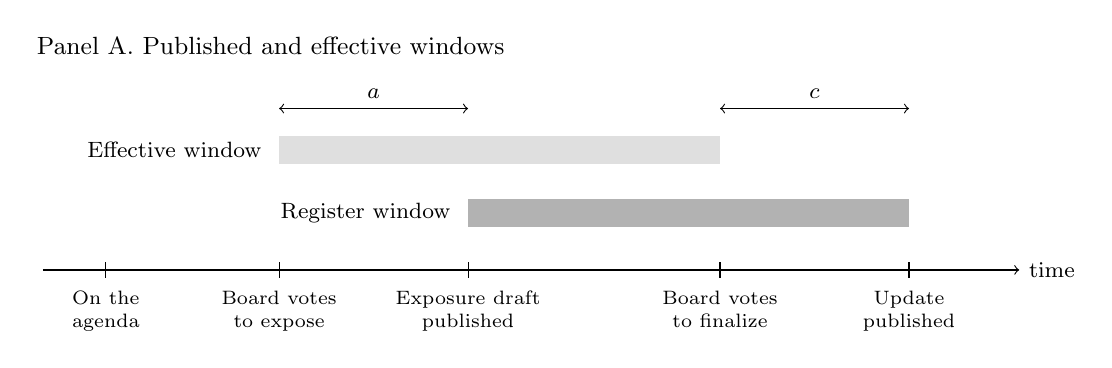
\begin{tikzpicture}[x=1cm,y=1cm,font=\footnotesize]
  \node[anchor=west,font=\small] at (-0.2,2.85) {Panel A. Published and effective windows};
  \draw[->] (0,0) -- (12.4,0) node[right] {time};
  \foreach \x/\lab in {0.8/{On the\\agenda}, 3.0/{Board votes\\to expose}, 5.4/{Exposure draft\\published}, 8.6/{Board votes\\to finalize}, 11.0/{Update\\published}}{
    \draw (\x,0.1) -- (\x,-0.1);
    \node[below,align=center,font=\scriptsize] at (\x,-0.15) {\lab};
  }
  \fill[gray!60] (5.4,0.55) rectangle (11.0,0.9);
  \node[left] at (5.3,0.725) {Register window};
  \fill[gray!25] (3.0,1.35) rectangle (8.6,1.7);
  \node[left] at (2.9,1.525) {Effective window};
  \draw[<->] (3.0,2.05) -- node[above] {$a$} (5.4,2.05);
  \draw[<->] (8.6,2.05) -- node[above] {$c$} (11.0,2.05);
\end{tikzpicture}

\vspace{1.5em}

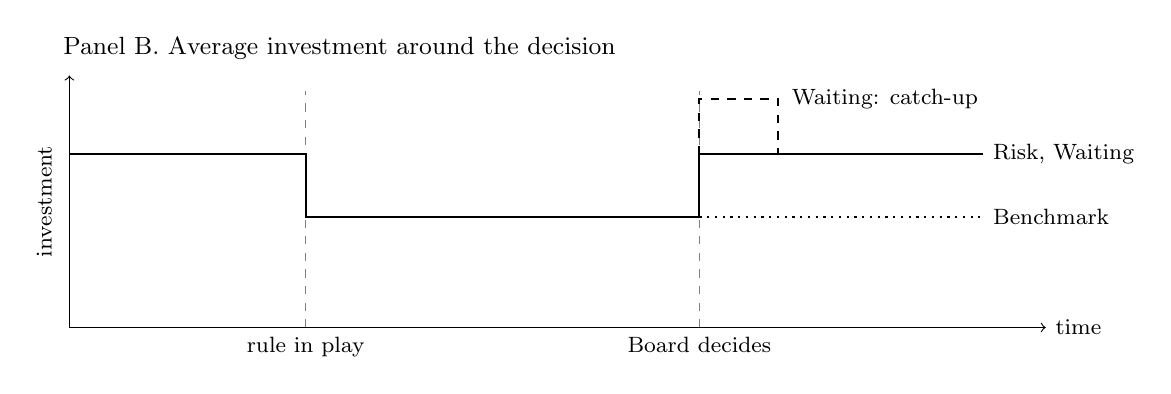
\begin{tikzpicture}[x=1cm,y=1cm,font=\footnotesize]
  \node[anchor=west,font=\small] at (-0.2,3.55) {Panel B. Average investment around the decision};
  \draw[->] (0,0) -- (12.4,0) node[right] {time};
  \draw[->] (0,0) -- (0,3.2);
  \node[rotate=90,anchor=south] at (-0.1,1.6) {investment};
  \draw[gray,dashed] (3,0) -- (3,3.0);
  \draw[gray,dashed] (8,0) -- (8,3.0);
  \node[below] at (3,0) {rule in play};
  \node[below] at (8,0) {Board decides};
  \draw[thick] (0,2.2) -- (3,2.2) -- (3,1.4) -- (8,1.4);
  \draw[thick,dotted] (8,1.4) -- (11.6,1.4) node[right] {Benchmark};
  \draw[thick] (8,1.4) -- (8,2.2) -- (11.6,2.2) node[right] {Risk, Waiting};
  \draw[thick,dashed] (8,2.2) -- (8,2.9) -- (9,2.9) -- (9,2.2);
  \node[right] at (9.05,2.9) {Waiting: catch-up};
\end{tikzpicture}
\caption{Pending Rules in the Model}\label{fig:model}
\par\medskip
\begin{minipage}{\linewidth}\footnotesize
\emph{Notes:} Panel A illustrates Proposition~\ref{prop:model:timing}. The register dates a proposal from the publication of its exposure draft to the publication of the final Update. In the model, the rule is effectively pending from the Board's decision to expose it to its decision to finalize it, which precede publication by $a$ and $c$ quarters. Panel B illustrates Propositions~\ref{prop:model:pending} and~\ref{prop:model:decision}. In the benchmark, investment falls only if the proposal is expected to worsen the reading, and on average it stays at the lower level once the Board decides. In both variants, the proposal leaves the expected reading unchanged; investment falls while the rule is pending and recovers when the Board decides, and in the waiting variant the postponed projects are undertaken at the decision. The pending level is drawn equal in the three cases for comparison.
\end{minipage}
\end{figure}

% ---------------------------------------------------------------------
\subsection{How the Manager Holds Back}\label{sec:model:holdback}

\begin{proposition}[Risk or waiting]\label{prop:model:holdback}
\leavevmode
\begin{enumerate}[label=(\roman*)]
  \item \emph{Investment opportunities.} In the risk variant, $\partial^{2}I_R/\partial\sigma^{2}\partial\gamma<0$ and $\partial^{2}\ln I_R/\partial\sigma^{2}\partial\gamma=0$. In the waiting variant, $\partial^{2}\ln I_W/\partial\sigma^{2}\partial\gamma>0$, and $\partial^{2}I_W/\partial\sigma^{2}\partial\gamma>0$ whenever fewer than a quarter of the projects are postponed.
  \item \emph{Irreversibility.} Suppose investment made while a proposal is pending can be adjusted after the decision at cost $\tfrac{k}{2}(\Delta I)^{2}$, and that $\theta$ is distributed symmetrically around $\bar\theta$. In the waiting variant, the share of projects postponed is $\lambda^{2}\sigma^{2}k/[(1+k)(A^{2}+\lambda^{2}\sigma^{2})]$, which increases in $k$. In the risk variant, the decline in investment is $Ax(1+k)/[1+k(1+x)]$ with $x\equiv\rho\lambda^{2}\sigma^{2}$; it equals $Ax$ up to terms of order $x^{2}$ for every $k$ and decreases slightly in $k$. Under the benchmark, investment is $A$ for every $k$.
  \item \emph{Catch-up.} In the waiting variant, postponed investment is undertaken when the Board decides. In the risk variant, there is none to undertake.
\end{enumerate}
\end{proposition}

Part~(i) holds because, in the waiting variant, a project with a high return loses more by waiting and is therefore less likely to be postponed. In the risk variant, the cost of uncertainty rises with the scale of investment, so firms with better opportunities cut more in levels and the same in proportion. Part~(ii) extends the familiar result that irreversibility raises the value of waiting \citep{dixit1994investment}. It holds in the waiting variant but not, to first order, in the risk variant. There, the ability to adjust after the decision makes the initial investment matter less in two ways at once, for expected value and for the exposure to the reading, and the two effects cancel to first order.

The evidence on these interactions was gathered to test other channels, but read through Proposition~\ref{prop:model:holdback} it favors waiting. The interaction of Pipeline Exposure with Tobin's $q$ in Table~\ref{tab:learning} is positive: 0.581 ($t=1.44$) for the investment rate and 0.651 ($t=2.12$) for total investment. The risk variant predicts a negative interaction in levels. The interaction with asset redeployability in Table~\ref{tab:realoptions} is also positive, 0.413 ($t=1.70$), as the waiting variant predicts and neither the risk variant nor the benchmark does, although it is not significant without oil and gas firms. % memo v7
The result that seems to point the other way is the absence of catch-up in the quarters after a standard is finalized. The catch-up test in Table~\ref{tab:realoptions}, however, begins in the quarter after the resolution quarter. The waiting variant predicts that postponed investment is undertaken as soon as the Board decides, which by Proposition~\ref{prop:model:timing} is typically before the Update is published. The catch-up would then fall in the resolution quarter or earlier, and part of it would be in the Resolving coefficient itself.

% ---------------------------------------------------------------------
\subsection{The Model and the Evidence}\label{sec:model:evidence}

Table~\ref{tab:model:evidence} sets the predictions of the benchmark and the two variants against the evidence. Three conclusions follow. First, the recovery when proposals are resolved rules out the anticipation benchmark and, with it, the view that firms simply price in what proposals are expected to require. Second, the ownership gradient locates the channel in how reported amounts are read rather than in cash flows. A pending rule could also lower investment because it changes the cash-flow payoff of irreversible investment, for example through compliance costs, or because preparing for it absorbs resources. Neither effect would depend on who holds the stock, and the second would persist after a standard is finalized. Third, between the two ways of holding back, the evidence favors waiting, provided that postponed investment returns when the Board decides. The results on the cost of capital and on price informativeness do not distinguish the benchmark from the two variants. They are the reason the model has no investor risk premia and no managerial learning from prices.

\begin{table}[tbp]
\centering
\caption{Predictions and Evidence}\label{tab:model:evidence}
\medskip
\small
\begin{tabular}{@{}lllccc@{}}
\toprule
 & & & \multicolumn{3}{c}{Prediction}\\
\cmidrule(l){4-6}
 & Estimate & Table & Benchmark & Risk & Waiting\\
\midrule
Investment while pending & $-1.531$ & \ref{tab:investment} & $-$\rlap{$^{a}$} & $-$ & $-$\\
Recovery at resolution (offset) & 0.88, 0.90 & \ref{tab:timing} & $0$ & $+$ & $+$\rlap{$^{b}$}\\
\addlinespace
\emph{Interaction with}\\
\quad transient (dedicated) ownership & $-1.012$ ($+0.609$) & \ref{tab:ownership} & $-$ ($+$)\rlap{$^{c}$} & $-$ ($+$) & $-$ ($+$)\\
\quad Tobin's $q$ & $+0.581$, $+0.651$ & \ref{tab:learning} & $0$ & $-$ & $+$\\
\quad asset redeployability & $+0.413$ & \ref{tab:realoptions} & $0$ & $0$ & $+$\\
\addlinespace
Catch-up after the resolution quarter & n.s. & \ref{tab:realoptions} & $0$ & $0$ & $0$\rlap{$^{d}$}\\
\bottomrule
\end{tabular}
% Estimates: memo v7.
\par\medskip
\begin{minipage}{\linewidth}\footnotesize
\emph{Notes:} Estimates are from the tables listed and are per standard deviation of Pipeline Exposure, multiplied by 1,000. The offset is the Resolving coefficient divided by minus the Active coefficient, in the resolution quarter and in the next. The two estimates for Tobin's $q$ are for the investment rate ($t=1.44$) and for total investment ($t=2.12$). The redeployability estimate has $t=1.70$ and is not significant without oil and gas firms. Predictions: Benchmark, Lemma~\ref{lem:model:benchmark}; Risk and Waiting, the two variants of Section~\ref{sec:model:setup}; the signs for Tobin's $q$ are for the level of investment. $^{a}$If proposals are expected to worsen the reading ($\bar\theta<\theta_0$). $^{b}$Including the catch-up of postponed projects when the Board decides (Proposition~\ref{prop:model:decision}). $^{c}$If the expected content of proposals affects investment through the reading. $^{d}$If postponed investment is undertaken when the Board decides, which Proposition~\ref{prop:model:timing} places in the resolution quarter or earlier; positive if it returns gradually.
\end{minipage}
\end{table}

% ---------------------------------------------------------------------
\subsection{Further Predictions}\label{sec:model:further}

The model makes predictions that the evidence so far does not test. Two of them concern the pipeline itself.

\begin{proposition}[Exposure portfolio]\label{prop:model:portfolio}
Let $e_{i,p,q}\equiv\sum_{o\in O_p}s_{i,o,q}/|O_p|$ be firm $i$'s exposure to proposal $p$, so that $\sum_{p\in P_q}e_{i,p,q}$ is Pipeline Exposure (Equation~\eqref{eq:components}). Suppose proposal $p$ shifts the firm's reading by $e_{i,p,q}\Delta_p$, where the $\Delta_p$ are independent with variances $\sigma_p^{2}$. Then the variance of the firm's reading is
\[
  \sigma_{i,q}^{2}=\sum_{p\in P_q}e_{i,p,q}^{2}\,\sigma_p^{2}.
\]
For a given Pipeline Exposure and equal $\sigma_p^{2}$, $\sigma_{i,q}^{2}$ increases with the concentration of exposure across proposals.
\end{proposition}

Pipeline Exposure is the sum of the weights $e_{i,p,q}$. By Propositions~\ref{prop:model:pending} and~\ref{prop:model:portfolio}, investment responds instead to the sum of their squares, weighted by the uncertainty of each proposal. Two firms with the same Pipeline Exposure should therefore respond differently if one of them has its exposure concentrated in a few proposals.

\begin{proposition}[Contested proposals]\label{prop:model:contested}
Suppose proposal $p$ is finalized with probability $\pi_p$, in which case it shifts the reading by $\Delta_p$, and is otherwise withdrawn. Then $\sigma_p^{2}=\pi_p(1-\pi_p)\Delta_p^{2}$, which is largest at $\pi_p=1/2$. The decline in investment in Proposition~\ref{prop:model:pending} is therefore largest for proposals that the Board could decide either way. Under the benchmark, the effect of the proposal, $\lambda\pi_p\Delta_p$, is monotone in $\pi_p$.
\end{proposition}

\begin{remark}[Expected time to decision]\label{rem:model:hazard}
Suppose a postponed project survives each quarter with probability $\phi_j$, discounting included, and the Board decides with probability $h$ per quarter. Waiting until the decision then retains the fraction $\delta_j=\phi_jh/[1-\phi_j(1-h)]$ of the project's value, which increases in $h$. In the waiting variant, a proposal therefore lowers investment more when a decision is expected soon. In the risk variant, the decline does not depend on $h$.
\end{remark}

These results and the earlier propositions point to seven tests, each with the data it requires.
\begin{itemize}
  \item \emph{Timing} (Proposition~\ref{prop:model:timing}). Date each proposal by the Board meetings at which it voted to expose the proposal and to finalize it, which the minutes record. With these dates, the Entering and Resolving coefficients should match the share of the quarter in which the rule is pending in the risk variant. In the waiting variant, investment should exceed that benchmark in the quarter of the decision.
  \item \emph{Concentration} (Proposition~\ref{prop:model:portfolio}). Add $\sum_p e_{i,p,q}^{2}\sigma_p^{2}$ to the investment regression. The model predicts that it carries the effect of Pipeline Exposure.
  \item \emph{Contestedness} (Proposition~\ref{prop:model:contested}). Code the position of each comment letter on its proposal, and whether the exposure draft carries the alternative views of dissenting Board members. The decline should be largest where support and opposition are balanced.
  \item \emph{Expected time to decision} (Remark~\ref{rem:model:hazard}). Code the stage of deliberation from the minutes. The waiting variant predicts larger declines as a decision approaches.
  \item \emph{Managerial incentives} (Propositions~\ref{prop:model:pending} and~\ref{prop:model:intensity}). Managers with equity that vests soon place more weight on the short-term price \citep{edmans2017equity}, which raises $\lambda$ in both variants. The risk variant adds that the decline should be steeper where managerial wealth is more sensitive to the stock price and flatter where compensation is convex \citep{core2002estimating}.
  \item \emph{Firms without traded equity} ($\lambda=0$). Firms that file a 10-K because of public debt but have no traded equity should show no decline, whereas channels that work through cash flows predict one \citep[compare][]{asker2015corporate}.
  \item \emph{The implementation window.} Between a final Update and its effective date, the rule is decided, so the model predicts no decline. A burden of implementation predicts one.
\end{itemize}

Each test uses data that the model, rather than the reduced-form evidence, identifies as relevant: when the Board decides rather than when it publishes, how contested a proposal is, how concentrated a firm's exposure is, and whether anyone reads the firm's reported amounts.


\appendix
\setcounter{section}{1}
% =====================================================================
% model_appendix.tex -- proofs for "A Model of Investment under a Pending Rule"
% Use: % =====================================================================
% model_appendix.tex -- proofs for "A Model of Investment under a Pending Rule"
% Use: % =====================================================================
% model_appendix.tex -- proofs for "A Model of Investment under a Pending Rule"
% Use: \input{model_appendix} inside the appendix. The algebra is checked
% symbolically in PipelineExposure/model_checks.py.
% =====================================================================

\section{Proofs for Section~\ref{sec:model}}\label{app:model}

Throughout, write $z\equiv\theta-\bar\theta$, so that $E[z]=0$ and $E[z^{2}]=\sigma^{2}$, and let
\[
  \Pi(\theta)\equiv\max_{I}\,\bigl[V(I)+\lambda\theta I\bigr]=\tfrac12(\gamma+\lambda\theta)^{2},
\]
attained at $I=\gamma+\lambda\theta$. Since $E[(\gamma+\lambda\theta)^{2}]=A^{2}+\lambda^{2}\sigma^{2}$, $E[\Pi(\theta)]=\tfrac12(A^{2}+\lambda^{2}\sigma^{2})$.

\paragraph{Proof of Lemma~\ref{lem:model:benchmark}.}
(i) With $\rho=0$, the manager maximizes $E[U(I;\theta)]=\gamma I-\tfrac12 I^{2}+\lambda\bar\theta I$, because $\varepsilon$ has mean zero. The objective is strictly concave, and the first-order condition gives $I=\gamma+\lambda\bar\theta=A$, which depends on the distribution of $\theta$ only through $\bar\theta$.

(ii) Once $\theta$ is known, investment is $\gamma+\lambda\theta$, so it changes by $\lambda(\theta-\bar\theta)=\lambda z$, whose expectation is zero.

(iii) Let the firm report $R=a+\theta I+\eta$, where $a\sim N(\bar a,\sigma_a^{2})$ is a component of firm value unrelated to the project and $\eta\sim N(0,\sigma_\eta^{2})$; $a$, $\eta$ and $\theta$ are mutually independent. Investors observe $R$ and the decided $\theta$ but not $a$ or $I$, and they conjecture investment $\hat I$. They set
\[
  P=E\bigl[a+V(I)\mid R,\theta\bigr]=\bar a+\beta\,(R-\bar a-\theta\hat I)+V(\hat I),\qquad
  \beta\equiv\frac{\sigma_a^{2}}{\sigma_a^{2}+\sigma_\eta^{2}},
\]
so that $P=\bar a+\beta(a-\bar a+\eta)+V(\hat I)+\beta\theta(I-\hat I)$. The manager chooses $I$ before $\theta$ is known and maximizes the mean minus $\rho/2$ times the variance of $(1-\omega)[a+V(I)]+\omega P$. The only term that depends on both $I$ and $\theta$ is $\omega\beta\theta(I-\hat I)$. Its variance is $\omega^{2}\beta^{2}\sigma^{2}(I-\hat I)^{2}$, and its covariance with the remaining random terms, which involve only $a$ and $\eta$, is zero. The first-order condition is
\[
  (1-\omega)(\gamma-I)+\omega\beta\bar\theta-\rho\,\omega^{2}\beta^{2}\sigma^{2}\,(I-\hat I)=0,
\]
and the objective is strictly concave in $I$. In equilibrium $I=\hat I$, so the last term vanishes and $\hat I=\gamma+\omega\beta\bar\theta/(1-\omega)$, which does not depend on $\sigma^{2}$. \qed

\paragraph{Proof of Proposition~\ref{prop:model:pending}.}
(i) Because $\varepsilon$ is independent of $\theta$, $\mathrm{Var}[U(I;\theta)]=\lambda^{2}\sigma^{2}I^{2}+\omega^{2}\mathrm{Var}(\varepsilon)$. The manager therefore maximizes $\gamma I-\tfrac12 I^{2}+\lambda\bar\theta I-\tfrac{\rho}{2}\lambda^{2}\sigma^{2}I^{2}$, which is strictly concave, and the first-order condition gives $I_R=A/(1+\rho\lambda^{2}\sigma^{2})$. Then
\[
  \frac{\partial I_R}{\partial\sigma^{2}}=-\frac{A\rho\lambda^{2}}{(1+\rho\lambda^{2}\sigma^{2})^{2}}<0\quad\text{for }\lambda\neq0.
\]

(ii) Undertaking project $j$ now yields $\max_I E[U(I;\theta)]=\tfrac12A^{2}$, by Lemma~\ref{lem:model:benchmark}(i). Postponing it yields $\delta_jE[\Pi(\theta)]=\tfrac12\delta_j(A^{2}+\lambda^{2}\sigma^{2})$. Hence the project is postponed if and only if $\delta_j>\delta^{*}$. Each project undertaken now invests $A$, and with $\delta_j$ uniform a mass $\delta^{*}$ of projects is undertaken, so $I_W=A\delta^{*}$ and
\[
  \frac{\partial I_W}{\partial\sigma^{2}}=-\frac{A^{3}\lambda^{2}}{(A^{2}+\lambda^{2}\sigma^{2})^{2}}<0\quad\text{for }\lambda\neq0.
\]
For a general distribution $G$ of $\delta_j$ with a positive density, $I_W=A\,G(\delta^{*})$, which decreases in $\sigma^{2}$ because $\delta^{*}$ does.

(iii) Set $\lambda=0$ in (i) and (ii). \qed

\paragraph{Proof of Proposition~\ref{prop:model:intensity}.}
(i) $A-I_R=A\rho\lambda^{2}\sigma^{2}/(1+\rho\lambda^{2}\sigma^{2})=A\rho\lambda^{2}\sigma^{2}+O(\sigma^{4})$ and $A-I_W=A\lambda^{2}\sigma^{2}/(A^{2}+\lambda^{2}\sigma^{2})=\lambda^{2}\sigma^{2}/A+O(\sigma^{4})$.

(ii) With $\bar\theta=0$, $A=\gamma$ and
\[
  \frac{\partial^{2}I_R}{\partial\sigma^{2}\partial\lambda}=-\frac{2\gamma\rho\lambda\,(1-\rho\lambda^{2}\sigma^{2})}{(1+\rho\lambda^{2}\sigma^{2})^{3}},\qquad
  \frac{\partial^{2}I_W}{\partial\sigma^{2}\partial\lambda}=-\frac{2\gamma^{3}\lambda\,(\gamma^{2}-\lambda^{2}\sigma^{2})}{(\gamma^{2}+\lambda^{2}\sigma^{2})^{3}}.
\]
For $\lambda>0$, the first is negative if and only if $\rho\lambda^{2}\sigma^{2}<1$, which is equivalent to $I_R>A/2$, and the second is negative if and only if $\lambda^{2}\sigma^{2}<\gamma^{2}$, which is equivalent to $\delta^{*}>1/2$. \qed

\paragraph{Proof of Proposition~\ref{prop:model:decision}.}
Once $\theta$ is known there is no uncertainty about the reading, so in both variants new investment maximizes $V(I)+\lambda\theta I$ and equals $\gamma+\lambda\theta$, whose mean is $A$. (i) The average recovery is therefore $A-I_R$, and no project was postponed. (ii) New investment recovers on average from $A\delta^{*}$ to $A$. Each postponed project is undertaken at the decision, because waiting longer only loses value. This adds a mass $1-\delta^{*}$ of projects, each of mean scale $A$, so investment in the period of the decision is on average $A(2-\delta^{*})>A$. (iii) follows from Lemma~\ref{lem:model:benchmark}(ii). \qed

\paragraph{Proof of Proposition~\ref{prop:model:timing}.}
Let $u\sim U[0,1]$ be the point in its quarter at which a document is published, and let $f$ be the share of a quarter in which the rule is effectively pending, so that investment in the quarter is lowered by $|\beta|f$. A proposal pending throughout the quarter has $f=1$, and each coefficient measures the difference from such a proposal, $|\beta|(1-E[f])$.

In the resolution quarter, the rule is effectively decided at $u-c$ if $u>c$ and in the previous quarter otherwise, so $f=\max\{0,u-c\}$ and
\[
  E[f]=\int_{c}^{1}(u-c)\,du=\tfrac12(1-c)^{2}.
\]
The Resolving coefficient is therefore $|\beta|[1-(1-c)^{2}/2]$. In the following quarter the resolved proposal has $f=0$, so the coefficient is $|\beta|$. In the issue quarter, the rule is effectively pending from $u-a$ if $u>a$ and throughout the quarter otherwise, so $f=1-\max\{0,u-a\}$, $E[f]=1-(1-a)^{2}/2$, and the Entering coefficient is $|\beta|(1-a)^{2}/2$. Setting $a=c=0$ gives (iii). In the waiting variant, the postponed projects are undertaken when the Board decides (Proposition~\ref{prop:model:decision}), which falls in the resolution quarter if $u>c$ and in the quarter before otherwise; this gives (iv).

With the estimates in Table~\ref{tab:timing}, $(1-a)^{2}/2=0.101/1.725$ and $1-(1-c)^{2}/2=1.518/1.725$ give $a=0.66$ and $c=0.51$, or 60 and 46 days at 91 days per quarter. % memo v7
\qed

\paragraph{Proof of Proposition~\ref{prop:model:holdback}.}
(i) Since $\partial A/\partial\gamma=1$, differentiating $\partial I_R/\partial\sigma^{2}=-A\rho\lambda^{2}/(1+\rho\lambda^{2}\sigma^{2})^{2}$ with respect to $\gamma$ gives $-\rho\lambda^{2}/(1+\rho\lambda^{2}\sigma^{2})^{2}<0$, and $\partial\ln I_R/\partial\sigma^{2}=-\rho\lambda^{2}/(1+\rho\lambda^{2}\sigma^{2})$ does not depend on $\gamma$. In the waiting variant, $\partial\ln I_W/\partial\sigma^{2}=-\lambda^{2}/(A^{2}+\lambda^{2}\sigma^{2})$, whose derivative with respect to $\gamma$ is $2A\lambda^{2}/(A^{2}+\lambda^{2}\sigma^{2})^{2}>0$, and
\[
  \frac{\partial^{2}I_W}{\partial\sigma^{2}\partial\gamma}=\frac{\lambda^{2}A^{2}\,(A^{2}-3\lambda^{2}\sigma^{2})}{(A^{2}+\lambda^{2}\sigma^{2})^{3}},
\]
which is positive if and only if $A^{2}>3\lambda^{2}\sigma^{2}$, that is, if and only if $1-\delta^{*}<1/4$.

(ii) Let the manager invest $I_0$ while the proposal is pending and, once $\theta$ is known, choose $I_1$ at adjustment cost $\tfrac{k}{2}(I_1-I_0)^{2}$, with $k>0$. Write $m\equiv\gamma+\lambda\theta=A+\lambda z$. The optimal adjustment is $I_1=(m+kI_0)/(1+k)$, and the resulting payoff is
\[
  \pi(z;I_0)=mI_0-\tfrac12I_0^{2}+\frac{(m-I_0)^{2}}{2(1+k)}.
\]
Hence
\[
  E[\pi]=AI_0-\tfrac12I_0^{2}+\frac{(A-I_0)^{2}+\lambda^{2}\sigma^{2}}{2(1+k)},
\]
which is maximized at $I_0=A$ with value $\tfrac12[A^{2}+\lambda^{2}\sigma^{2}/(1+k)]$. This proves the claim for the benchmark. In the waiting variant, postponing project $j$ still yields $\tfrac12\delta_j(A^{2}+\lambda^{2}\sigma^{2})$, so the project is postponed if and only if
\[
  \delta_j>\frac{A^{2}+\lambda^{2}\sigma^{2}/(1+k)}{A^{2}+\lambda^{2}\sigma^{2}},
\]
and the share postponed is $\lambda^{2}\sigma^{2}k/[(1+k)(A^{2}+\lambda^{2}\sigma^{2})]$. Its derivative with respect to $k$ is $\lambda^{2}\sigma^{2}/[(1+k)^{2}(A^{2}+\lambda^{2}\sigma^{2})]>0$.

In the risk variant, $\pi$ is quadratic in $z$, with linear coefficient $c_1=\lambda(A+kI_0)/(1+k)$ and quadratic coefficient $c_2=\lambda^{2}/[2(1+k)]$. Because $z$ is symmetric, $E[z^{3}]=0$ and $\mathrm{Var}[\pi]=c_1^{2}\sigma^{2}+c_2^{2}\,\mathrm{Var}(z^{2})$, in which only $c_1$ depends on $I_0$. The objective $E[\pi]-\tfrac{\rho}{2}\mathrm{Var}[\pi]$ is strictly concave in $I_0$, and its first-order condition,
\[
  \frac{k}{1+k}(A-I_0)-\rho\sigma^{2}c_1\,\frac{\lambda k}{1+k}=0,
\]
gives $I_0=A(1+k-x)/[1+k(1+x)]$ with $x\equiv\rho\lambda^{2}\sigma^{2}$. Hence
\[
  A-I_0=\frac{Ax(1+k)}{1+k(1+x)}=Ax-\frac{Ax^{2}k}{1+k}+O(x^{3}),\qquad
  \frac{\partial(A-I_0)}{\partial k}=-\frac{Ax^{2}}{[1+k(1+x)]^{2}}<0.
\]

(iii) follows from Proposition~\ref{prop:model:decision}. \qed

\paragraph{Proof of Proposition~\ref{prop:model:portfolio}.}
The shift in the firm's reading is $\sum_{p}e_{i,p,q}\Delta_p$, whose variance is $\sum_{p}e_{i,p,q}^{2}\sigma_p^{2}$ because the $\Delta_p$ are independent. With $\sigma_p^{2}=\sigma^{2}$ for all $p$ and Pipeline Exposure $X_{i,q}\equiv\sum_pe_{i,p,q}$ held fixed, $\sigma_{i,q}^{2}=\sigma^{2}X_{i,q}^{2}H_{i,q}$, where $H_{i,q}\equiv\sum_p(e_{i,p,q}/X_{i,q})^{2}$ is the Herfindahl index of the firm's exposure across proposals. \qed

\paragraph{Proof of Proposition~\ref{prop:model:contested}.}
The shift is $\Delta_p$ with probability $\pi_p$ and zero otherwise. Its variance, $\pi_p(1-\pi_p)\Delta_p^{2}$, is largest at $\pi_p=1/2$, and the decline in Proposition~\ref{prop:model:pending} increases in the variance. Its mean is $\pi_p\Delta_p$, so under the benchmark investment moves by $\lambda(\bar\theta-\theta_0)=\lambda\pi_p\Delta_p$, which is monotone in $\pi_p$. \qed

\paragraph{Proof of Remark~\ref{rem:model:hazard}.}
While the proposal is pending the problem is stationary, so a manager who prefers to wait in one quarter prefers to wait in every later quarter until the Board decides. The value $W_j$ of holding project $j$ then satisfies $W_j=\phi_j\{hE[\Pi(\theta)]+(1-h)W_j\}$, so $W_j=\delta_jE[\Pi(\theta)]$ with $\delta_j=\phi_jh/[1-\phi_j(1-h)]$, and
\[
  \frac{\partial\delta_j}{\partial h}=\frac{\phi_j(1-\phi_j)}{[1-\phi_j(1-h)]^{2}}>0.
\]
The project is postponed if and only if $\delta_j>\delta^{*}$, that is, if and only if $\phi_j>\delta^{*}/[\delta^{*}+h(1-\delta^{*})]$. This threshold decreases in $h$, so for any distribution of $\phi_j$ with a positive density the share of projects postponed increases in $h$. In the risk variant, $I_R$ does not depend on $h$. \qed
 inside the appendix. The algebra is checked
% symbolically in PipelineExposure/model_checks.py.
% =====================================================================

\section{Proofs for Section~\ref{sec:model}}\label{app:model}

Throughout, write $z\equiv\theta-\bar\theta$, so that $E[z]=0$ and $E[z^{2}]=\sigma^{2}$, and let
\[
  \Pi(\theta)\equiv\max_{I}\,\bigl[V(I)+\lambda\theta I\bigr]=\tfrac12(\gamma+\lambda\theta)^{2},
\]
attained at $I=\gamma+\lambda\theta$. Since $E[(\gamma+\lambda\theta)^{2}]=A^{2}+\lambda^{2}\sigma^{2}$, $E[\Pi(\theta)]=\tfrac12(A^{2}+\lambda^{2}\sigma^{2})$.

\paragraph{Proof of Lemma~\ref{lem:model:benchmark}.}
(i) With $\rho=0$, the manager maximizes $E[U(I;\theta)]=\gamma I-\tfrac12 I^{2}+\lambda\bar\theta I$, because $\varepsilon$ has mean zero. The objective is strictly concave, and the first-order condition gives $I=\gamma+\lambda\bar\theta=A$, which depends on the distribution of $\theta$ only through $\bar\theta$.

(ii) Once $\theta$ is known, investment is $\gamma+\lambda\theta$, so it changes by $\lambda(\theta-\bar\theta)=\lambda z$, whose expectation is zero.

(iii) Let the firm report $R=a+\theta I+\eta$, where $a\sim N(\bar a,\sigma_a^{2})$ is a component of firm value unrelated to the project and $\eta\sim N(0,\sigma_\eta^{2})$; $a$, $\eta$ and $\theta$ are mutually independent. Investors observe $R$ and the decided $\theta$ but not $a$ or $I$, and they conjecture investment $\hat I$. They set
\[
  P=E\bigl[a+V(I)\mid R,\theta\bigr]=\bar a+\beta\,(R-\bar a-\theta\hat I)+V(\hat I),\qquad
  \beta\equiv\frac{\sigma_a^{2}}{\sigma_a^{2}+\sigma_\eta^{2}},
\]
so that $P=\bar a+\beta(a-\bar a+\eta)+V(\hat I)+\beta\theta(I-\hat I)$. The manager chooses $I$ before $\theta$ is known and maximizes the mean minus $\rho/2$ times the variance of $(1-\omega)[a+V(I)]+\omega P$. The only term that depends on both $I$ and $\theta$ is $\omega\beta\theta(I-\hat I)$. Its variance is $\omega^{2}\beta^{2}\sigma^{2}(I-\hat I)^{2}$, and its covariance with the remaining random terms, which involve only $a$ and $\eta$, is zero. The first-order condition is
\[
  (1-\omega)(\gamma-I)+\omega\beta\bar\theta-\rho\,\omega^{2}\beta^{2}\sigma^{2}\,(I-\hat I)=0,
\]
and the objective is strictly concave in $I$. In equilibrium $I=\hat I$, so the last term vanishes and $\hat I=\gamma+\omega\beta\bar\theta/(1-\omega)$, which does not depend on $\sigma^{2}$. \qed

\paragraph{Proof of Proposition~\ref{prop:model:pending}.}
(i) Because $\varepsilon$ is independent of $\theta$, $\mathrm{Var}[U(I;\theta)]=\lambda^{2}\sigma^{2}I^{2}+\omega^{2}\mathrm{Var}(\varepsilon)$. The manager therefore maximizes $\gamma I-\tfrac12 I^{2}+\lambda\bar\theta I-\tfrac{\rho}{2}\lambda^{2}\sigma^{2}I^{2}$, which is strictly concave, and the first-order condition gives $I_R=A/(1+\rho\lambda^{2}\sigma^{2})$. Then
\[
  \frac{\partial I_R}{\partial\sigma^{2}}=-\frac{A\rho\lambda^{2}}{(1+\rho\lambda^{2}\sigma^{2})^{2}}<0\quad\text{for }\lambda\neq0.
\]

(ii) Undertaking project $j$ now yields $\max_I E[U(I;\theta)]=\tfrac12A^{2}$, by Lemma~\ref{lem:model:benchmark}(i). Postponing it yields $\delta_jE[\Pi(\theta)]=\tfrac12\delta_j(A^{2}+\lambda^{2}\sigma^{2})$. Hence the project is postponed if and only if $\delta_j>\delta^{*}$. Each project undertaken now invests $A$, and with $\delta_j$ uniform a mass $\delta^{*}$ of projects is undertaken, so $I_W=A\delta^{*}$ and
\[
  \frac{\partial I_W}{\partial\sigma^{2}}=-\frac{A^{3}\lambda^{2}}{(A^{2}+\lambda^{2}\sigma^{2})^{2}}<0\quad\text{for }\lambda\neq0.
\]
For a general distribution $G$ of $\delta_j$ with a positive density, $I_W=A\,G(\delta^{*})$, which decreases in $\sigma^{2}$ because $\delta^{*}$ does.

(iii) Set $\lambda=0$ in (i) and (ii). \qed

\paragraph{Proof of Proposition~\ref{prop:model:intensity}.}
(i) $A-I_R=A\rho\lambda^{2}\sigma^{2}/(1+\rho\lambda^{2}\sigma^{2})=A\rho\lambda^{2}\sigma^{2}+O(\sigma^{4})$ and $A-I_W=A\lambda^{2}\sigma^{2}/(A^{2}+\lambda^{2}\sigma^{2})=\lambda^{2}\sigma^{2}/A+O(\sigma^{4})$.

(ii) With $\bar\theta=0$, $A=\gamma$ and
\[
  \frac{\partial^{2}I_R}{\partial\sigma^{2}\partial\lambda}=-\frac{2\gamma\rho\lambda\,(1-\rho\lambda^{2}\sigma^{2})}{(1+\rho\lambda^{2}\sigma^{2})^{3}},\qquad
  \frac{\partial^{2}I_W}{\partial\sigma^{2}\partial\lambda}=-\frac{2\gamma^{3}\lambda\,(\gamma^{2}-\lambda^{2}\sigma^{2})}{(\gamma^{2}+\lambda^{2}\sigma^{2})^{3}}.
\]
For $\lambda>0$, the first is negative if and only if $\rho\lambda^{2}\sigma^{2}<1$, which is equivalent to $I_R>A/2$, and the second is negative if and only if $\lambda^{2}\sigma^{2}<\gamma^{2}$, which is equivalent to $\delta^{*}>1/2$. \qed

\paragraph{Proof of Proposition~\ref{prop:model:decision}.}
Once $\theta$ is known there is no uncertainty about the reading, so in both variants new investment maximizes $V(I)+\lambda\theta I$ and equals $\gamma+\lambda\theta$, whose mean is $A$. (i) The average recovery is therefore $A-I_R$, and no project was postponed. (ii) New investment recovers on average from $A\delta^{*}$ to $A$. Each postponed project is undertaken at the decision, because waiting longer only loses value. This adds a mass $1-\delta^{*}$ of projects, each of mean scale $A$, so investment in the period of the decision is on average $A(2-\delta^{*})>A$. (iii) follows from Lemma~\ref{lem:model:benchmark}(ii). \qed

\paragraph{Proof of Proposition~\ref{prop:model:timing}.}
Let $u\sim U[0,1]$ be the point in its quarter at which a document is published, and let $f$ be the share of a quarter in which the rule is effectively pending, so that investment in the quarter is lowered by $|\beta|f$. A proposal pending throughout the quarter has $f=1$, and each coefficient measures the difference from such a proposal, $|\beta|(1-E[f])$.

In the resolution quarter, the rule is effectively decided at $u-c$ if $u>c$ and in the previous quarter otherwise, so $f=\max\{0,u-c\}$ and
\[
  E[f]=\int_{c}^{1}(u-c)\,du=\tfrac12(1-c)^{2}.
\]
The Resolving coefficient is therefore $|\beta|[1-(1-c)^{2}/2]$. In the following quarter the resolved proposal has $f=0$, so the coefficient is $|\beta|$. In the issue quarter, the rule is effectively pending from $u-a$ if $u>a$ and throughout the quarter otherwise, so $f=1-\max\{0,u-a\}$, $E[f]=1-(1-a)^{2}/2$, and the Entering coefficient is $|\beta|(1-a)^{2}/2$. Setting $a=c=0$ gives (iii). In the waiting variant, the postponed projects are undertaken when the Board decides (Proposition~\ref{prop:model:decision}), which falls in the resolution quarter if $u>c$ and in the quarter before otherwise; this gives (iv).

With the estimates in Table~\ref{tab:timing}, $(1-a)^{2}/2=0.101/1.725$ and $1-(1-c)^{2}/2=1.518/1.725$ give $a=0.66$ and $c=0.51$, or 60 and 46 days at 91 days per quarter. % memo v7
\qed

\paragraph{Proof of Proposition~\ref{prop:model:holdback}.}
(i) Since $\partial A/\partial\gamma=1$, differentiating $\partial I_R/\partial\sigma^{2}=-A\rho\lambda^{2}/(1+\rho\lambda^{2}\sigma^{2})^{2}$ with respect to $\gamma$ gives $-\rho\lambda^{2}/(1+\rho\lambda^{2}\sigma^{2})^{2}<0$, and $\partial\ln I_R/\partial\sigma^{2}=-\rho\lambda^{2}/(1+\rho\lambda^{2}\sigma^{2})$ does not depend on $\gamma$. In the waiting variant, $\partial\ln I_W/\partial\sigma^{2}=-\lambda^{2}/(A^{2}+\lambda^{2}\sigma^{2})$, whose derivative with respect to $\gamma$ is $2A\lambda^{2}/(A^{2}+\lambda^{2}\sigma^{2})^{2}>0$, and
\[
  \frac{\partial^{2}I_W}{\partial\sigma^{2}\partial\gamma}=\frac{\lambda^{2}A^{2}\,(A^{2}-3\lambda^{2}\sigma^{2})}{(A^{2}+\lambda^{2}\sigma^{2})^{3}},
\]
which is positive if and only if $A^{2}>3\lambda^{2}\sigma^{2}$, that is, if and only if $1-\delta^{*}<1/4$.

(ii) Let the manager invest $I_0$ while the proposal is pending and, once $\theta$ is known, choose $I_1$ at adjustment cost $\tfrac{k}{2}(I_1-I_0)^{2}$, with $k>0$. Write $m\equiv\gamma+\lambda\theta=A+\lambda z$. The optimal adjustment is $I_1=(m+kI_0)/(1+k)$, and the resulting payoff is
\[
  \pi(z;I_0)=mI_0-\tfrac12I_0^{2}+\frac{(m-I_0)^{2}}{2(1+k)}.
\]
Hence
\[
  E[\pi]=AI_0-\tfrac12I_0^{2}+\frac{(A-I_0)^{2}+\lambda^{2}\sigma^{2}}{2(1+k)},
\]
which is maximized at $I_0=A$ with value $\tfrac12[A^{2}+\lambda^{2}\sigma^{2}/(1+k)]$. This proves the claim for the benchmark. In the waiting variant, postponing project $j$ still yields $\tfrac12\delta_j(A^{2}+\lambda^{2}\sigma^{2})$, so the project is postponed if and only if
\[
  \delta_j>\frac{A^{2}+\lambda^{2}\sigma^{2}/(1+k)}{A^{2}+\lambda^{2}\sigma^{2}},
\]
and the share postponed is $\lambda^{2}\sigma^{2}k/[(1+k)(A^{2}+\lambda^{2}\sigma^{2})]$. Its derivative with respect to $k$ is $\lambda^{2}\sigma^{2}/[(1+k)^{2}(A^{2}+\lambda^{2}\sigma^{2})]>0$.

In the risk variant, $\pi$ is quadratic in $z$, with linear coefficient $c_1=\lambda(A+kI_0)/(1+k)$ and quadratic coefficient $c_2=\lambda^{2}/[2(1+k)]$. Because $z$ is symmetric, $E[z^{3}]=0$ and $\mathrm{Var}[\pi]=c_1^{2}\sigma^{2}+c_2^{2}\,\mathrm{Var}(z^{2})$, in which only $c_1$ depends on $I_0$. The objective $E[\pi]-\tfrac{\rho}{2}\mathrm{Var}[\pi]$ is strictly concave in $I_0$, and its first-order condition,
\[
  \frac{k}{1+k}(A-I_0)-\rho\sigma^{2}c_1\,\frac{\lambda k}{1+k}=0,
\]
gives $I_0=A(1+k-x)/[1+k(1+x)]$ with $x\equiv\rho\lambda^{2}\sigma^{2}$. Hence
\[
  A-I_0=\frac{Ax(1+k)}{1+k(1+x)}=Ax-\frac{Ax^{2}k}{1+k}+O(x^{3}),\qquad
  \frac{\partial(A-I_0)}{\partial k}=-\frac{Ax^{2}}{[1+k(1+x)]^{2}}<0.
\]

(iii) follows from Proposition~\ref{prop:model:decision}. \qed

\paragraph{Proof of Proposition~\ref{prop:model:portfolio}.}
The shift in the firm's reading is $\sum_{p}e_{i,p,q}\Delta_p$, whose variance is $\sum_{p}e_{i,p,q}^{2}\sigma_p^{2}$ because the $\Delta_p$ are independent. With $\sigma_p^{2}=\sigma^{2}$ for all $p$ and Pipeline Exposure $X_{i,q}\equiv\sum_pe_{i,p,q}$ held fixed, $\sigma_{i,q}^{2}=\sigma^{2}X_{i,q}^{2}H_{i,q}$, where $H_{i,q}\equiv\sum_p(e_{i,p,q}/X_{i,q})^{2}$ is the Herfindahl index of the firm's exposure across proposals. \qed

\paragraph{Proof of Proposition~\ref{prop:model:contested}.}
The shift is $\Delta_p$ with probability $\pi_p$ and zero otherwise. Its variance, $\pi_p(1-\pi_p)\Delta_p^{2}$, is largest at $\pi_p=1/2$, and the decline in Proposition~\ref{prop:model:pending} increases in the variance. Its mean is $\pi_p\Delta_p$, so under the benchmark investment moves by $\lambda(\bar\theta-\theta_0)=\lambda\pi_p\Delta_p$, which is monotone in $\pi_p$. \qed

\paragraph{Proof of Remark~\ref{rem:model:hazard}.}
While the proposal is pending the problem is stationary, so a manager who prefers to wait in one quarter prefers to wait in every later quarter until the Board decides. The value $W_j$ of holding project $j$ then satisfies $W_j=\phi_j\{hE[\Pi(\theta)]+(1-h)W_j\}$, so $W_j=\delta_jE[\Pi(\theta)]$ with $\delta_j=\phi_jh/[1-\phi_j(1-h)]$, and
\[
  \frac{\partial\delta_j}{\partial h}=\frac{\phi_j(1-\phi_j)}{[1-\phi_j(1-h)]^{2}}>0.
\]
The project is postponed if and only if $\delta_j>\delta^{*}$, that is, if and only if $\phi_j>\delta^{*}/[\delta^{*}+h(1-\delta^{*})]$. This threshold decreases in $h$, so for any distribution of $\phi_j$ with a positive density the share of projects postponed increases in $h$. In the risk variant, $I_R$ does not depend on $h$. \qed
 inside the appendix. The algebra is checked
% symbolically in PipelineExposure/model_checks.py.
% =====================================================================

\section{Proofs for Section~\ref{sec:model}}\label{app:model}

Throughout, write $z\equiv\theta-\bar\theta$, so that $E[z]=0$ and $E[z^{2}]=\sigma^{2}$, and let
\[
  \Pi(\theta)\equiv\max_{I}\,\bigl[V(I)+\lambda\theta I\bigr]=\tfrac12(\gamma+\lambda\theta)^{2},
\]
attained at $I=\gamma+\lambda\theta$. Since $E[(\gamma+\lambda\theta)^{2}]=A^{2}+\lambda^{2}\sigma^{2}$, $E[\Pi(\theta)]=\tfrac12(A^{2}+\lambda^{2}\sigma^{2})$.

\paragraph{Proof of Lemma~\ref{lem:model:benchmark}.}
(i) With $\rho=0$, the manager maximizes $E[U(I;\theta)]=\gamma I-\tfrac12 I^{2}+\lambda\bar\theta I$, because $\varepsilon$ has mean zero. The objective is strictly concave, and the first-order condition gives $I=\gamma+\lambda\bar\theta=A$, which depends on the distribution of $\theta$ only through $\bar\theta$.

(ii) Once $\theta$ is known, investment is $\gamma+\lambda\theta$, so it changes by $\lambda(\theta-\bar\theta)=\lambda z$, whose expectation is zero.

(iii) Let the firm report $R=a+\theta I+\eta$, where $a\sim N(\bar a,\sigma_a^{2})$ is a component of firm value unrelated to the project and $\eta\sim N(0,\sigma_\eta^{2})$; $a$, $\eta$ and $\theta$ are mutually independent. Investors observe $R$ and the decided $\theta$ but not $a$ or $I$, and they conjecture investment $\hat I$. They set
\[
  P=E\bigl[a+V(I)\mid R,\theta\bigr]=\bar a+\beta\,(R-\bar a-\theta\hat I)+V(\hat I),\qquad
  \beta\equiv\frac{\sigma_a^{2}}{\sigma_a^{2}+\sigma_\eta^{2}},
\]
so that $P=\bar a+\beta(a-\bar a+\eta)+V(\hat I)+\beta\theta(I-\hat I)$. The manager chooses $I$ before $\theta$ is known and maximizes the mean minus $\rho/2$ times the variance of $(1-\omega)[a+V(I)]+\omega P$. The only term that depends on both $I$ and $\theta$ is $\omega\beta\theta(I-\hat I)$. Its variance is $\omega^{2}\beta^{2}\sigma^{2}(I-\hat I)^{2}$, and its covariance with the remaining random terms, which involve only $a$ and $\eta$, is zero. The first-order condition is
\[
  (1-\omega)(\gamma-I)+\omega\beta\bar\theta-\rho\,\omega^{2}\beta^{2}\sigma^{2}\,(I-\hat I)=0,
\]
and the objective is strictly concave in $I$. In equilibrium $I=\hat I$, so the last term vanishes and $\hat I=\gamma+\omega\beta\bar\theta/(1-\omega)$, which does not depend on $\sigma^{2}$. \qed

\paragraph{Proof of Proposition~\ref{prop:model:pending}.}
(i) Because $\varepsilon$ is independent of $\theta$, $\mathrm{Var}[U(I;\theta)]=\lambda^{2}\sigma^{2}I^{2}+\omega^{2}\mathrm{Var}(\varepsilon)$. The manager therefore maximizes $\gamma I-\tfrac12 I^{2}+\lambda\bar\theta I-\tfrac{\rho}{2}\lambda^{2}\sigma^{2}I^{2}$, which is strictly concave, and the first-order condition gives $I_R=A/(1+\rho\lambda^{2}\sigma^{2})$. Then
\[
  \frac{\partial I_R}{\partial\sigma^{2}}=-\frac{A\rho\lambda^{2}}{(1+\rho\lambda^{2}\sigma^{2})^{2}}<0\quad\text{for }\lambda\neq0.
\]

(ii) Undertaking project $j$ now yields $\max_I E[U(I;\theta)]=\tfrac12A^{2}$, by Lemma~\ref{lem:model:benchmark}(i). Postponing it yields $\delta_jE[\Pi(\theta)]=\tfrac12\delta_j(A^{2}+\lambda^{2}\sigma^{2})$. Hence the project is postponed if and only if $\delta_j>\delta^{*}$. Each project undertaken now invests $A$, and with $\delta_j$ uniform a mass $\delta^{*}$ of projects is undertaken, so $I_W=A\delta^{*}$ and
\[
  \frac{\partial I_W}{\partial\sigma^{2}}=-\frac{A^{3}\lambda^{2}}{(A^{2}+\lambda^{2}\sigma^{2})^{2}}<0\quad\text{for }\lambda\neq0.
\]
For a general distribution $G$ of $\delta_j$ with a positive density, $I_W=A\,G(\delta^{*})$, which decreases in $\sigma^{2}$ because $\delta^{*}$ does.

(iii) Set $\lambda=0$ in (i) and (ii). \qed

\paragraph{Proof of Proposition~\ref{prop:model:intensity}.}
(i) $A-I_R=A\rho\lambda^{2}\sigma^{2}/(1+\rho\lambda^{2}\sigma^{2})=A\rho\lambda^{2}\sigma^{2}+O(\sigma^{4})$ and $A-I_W=A\lambda^{2}\sigma^{2}/(A^{2}+\lambda^{2}\sigma^{2})=\lambda^{2}\sigma^{2}/A+O(\sigma^{4})$.

(ii) With $\bar\theta=0$, $A=\gamma$ and
\[
  \frac{\partial^{2}I_R}{\partial\sigma^{2}\partial\lambda}=-\frac{2\gamma\rho\lambda\,(1-\rho\lambda^{2}\sigma^{2})}{(1+\rho\lambda^{2}\sigma^{2})^{3}},\qquad
  \frac{\partial^{2}I_W}{\partial\sigma^{2}\partial\lambda}=-\frac{2\gamma^{3}\lambda\,(\gamma^{2}-\lambda^{2}\sigma^{2})}{(\gamma^{2}+\lambda^{2}\sigma^{2})^{3}}.
\]
For $\lambda>0$, the first is negative if and only if $\rho\lambda^{2}\sigma^{2}<1$, which is equivalent to $I_R>A/2$, and the second is negative if and only if $\lambda^{2}\sigma^{2}<\gamma^{2}$, which is equivalent to $\delta^{*}>1/2$. \qed

\paragraph{Proof of Proposition~\ref{prop:model:decision}.}
Once $\theta$ is known there is no uncertainty about the reading, so in both variants new investment maximizes $V(I)+\lambda\theta I$ and equals $\gamma+\lambda\theta$, whose mean is $A$. (i) The average recovery is therefore $A-I_R$, and no project was postponed. (ii) New investment recovers on average from $A\delta^{*}$ to $A$. Each postponed project is undertaken at the decision, because waiting longer only loses value. This adds a mass $1-\delta^{*}$ of projects, each of mean scale $A$, so investment in the period of the decision is on average $A(2-\delta^{*})>A$. (iii) follows from Lemma~\ref{lem:model:benchmark}(ii). \qed

\paragraph{Proof of Proposition~\ref{prop:model:timing}.}
Let $u\sim U[0,1]$ be the point in its quarter at which a document is published, and let $f$ be the share of a quarter in which the rule is effectively pending, so that investment in the quarter is lowered by $|\beta|f$. A proposal pending throughout the quarter has $f=1$, and each coefficient measures the difference from such a proposal, $|\beta|(1-E[f])$.

In the resolution quarter, the rule is effectively decided at $u-c$ if $u>c$ and in the previous quarter otherwise, so $f=\max\{0,u-c\}$ and
\[
  E[f]=\int_{c}^{1}(u-c)\,du=\tfrac12(1-c)^{2}.
\]
The Resolving coefficient is therefore $|\beta|[1-(1-c)^{2}/2]$. In the following quarter the resolved proposal has $f=0$, so the coefficient is $|\beta|$. In the issue quarter, the rule is effectively pending from $u-a$ if $u>a$ and throughout the quarter otherwise, so $f=1-\max\{0,u-a\}$, $E[f]=1-(1-a)^{2}/2$, and the Entering coefficient is $|\beta|(1-a)^{2}/2$. Setting $a=c=0$ gives (iii). In the waiting variant, the postponed projects are undertaken when the Board decides (Proposition~\ref{prop:model:decision}), which falls in the resolution quarter if $u>c$ and in the quarter before otherwise; this gives (iv).

With the estimates in Table~\ref{tab:timing}, $(1-a)^{2}/2=0.101/1.725$ and $1-(1-c)^{2}/2=1.518/1.725$ give $a=0.66$ and $c=0.51$, or 60 and 46 days at 91 days per quarter. % memo v7
\qed

\paragraph{Proof of Proposition~\ref{prop:model:holdback}.}
(i) Since $\partial A/\partial\gamma=1$, differentiating $\partial I_R/\partial\sigma^{2}=-A\rho\lambda^{2}/(1+\rho\lambda^{2}\sigma^{2})^{2}$ with respect to $\gamma$ gives $-\rho\lambda^{2}/(1+\rho\lambda^{2}\sigma^{2})^{2}<0$, and $\partial\ln I_R/\partial\sigma^{2}=-\rho\lambda^{2}/(1+\rho\lambda^{2}\sigma^{2})$ does not depend on $\gamma$. In the waiting variant, $\partial\ln I_W/\partial\sigma^{2}=-\lambda^{2}/(A^{2}+\lambda^{2}\sigma^{2})$, whose derivative with respect to $\gamma$ is $2A\lambda^{2}/(A^{2}+\lambda^{2}\sigma^{2})^{2}>0$, and
\[
  \frac{\partial^{2}I_W}{\partial\sigma^{2}\partial\gamma}=\frac{\lambda^{2}A^{2}\,(A^{2}-3\lambda^{2}\sigma^{2})}{(A^{2}+\lambda^{2}\sigma^{2})^{3}},
\]
which is positive if and only if $A^{2}>3\lambda^{2}\sigma^{2}$, that is, if and only if $1-\delta^{*}<1/4$.

(ii) Let the manager invest $I_0$ while the proposal is pending and, once $\theta$ is known, choose $I_1$ at adjustment cost $\tfrac{k}{2}(I_1-I_0)^{2}$, with $k>0$. Write $m\equiv\gamma+\lambda\theta=A+\lambda z$. The optimal adjustment is $I_1=(m+kI_0)/(1+k)$, and the resulting payoff is
\[
  \pi(z;I_0)=mI_0-\tfrac12I_0^{2}+\frac{(m-I_0)^{2}}{2(1+k)}.
\]
Hence
\[
  E[\pi]=AI_0-\tfrac12I_0^{2}+\frac{(A-I_0)^{2}+\lambda^{2}\sigma^{2}}{2(1+k)},
\]
which is maximized at $I_0=A$ with value $\tfrac12[A^{2}+\lambda^{2}\sigma^{2}/(1+k)]$. This proves the claim for the benchmark. In the waiting variant, postponing project $j$ still yields $\tfrac12\delta_j(A^{2}+\lambda^{2}\sigma^{2})$, so the project is postponed if and only if
\[
  \delta_j>\frac{A^{2}+\lambda^{2}\sigma^{2}/(1+k)}{A^{2}+\lambda^{2}\sigma^{2}},
\]
and the share postponed is $\lambda^{2}\sigma^{2}k/[(1+k)(A^{2}+\lambda^{2}\sigma^{2})]$. Its derivative with respect to $k$ is $\lambda^{2}\sigma^{2}/[(1+k)^{2}(A^{2}+\lambda^{2}\sigma^{2})]>0$.

In the risk variant, $\pi$ is quadratic in $z$, with linear coefficient $c_1=\lambda(A+kI_0)/(1+k)$ and quadratic coefficient $c_2=\lambda^{2}/[2(1+k)]$. Because $z$ is symmetric, $E[z^{3}]=0$ and $\mathrm{Var}[\pi]=c_1^{2}\sigma^{2}+c_2^{2}\,\mathrm{Var}(z^{2})$, in which only $c_1$ depends on $I_0$. The objective $E[\pi]-\tfrac{\rho}{2}\mathrm{Var}[\pi]$ is strictly concave in $I_0$, and its first-order condition,
\[
  \frac{k}{1+k}(A-I_0)-\rho\sigma^{2}c_1\,\frac{\lambda k}{1+k}=0,
\]
gives $I_0=A(1+k-x)/[1+k(1+x)]$ with $x\equiv\rho\lambda^{2}\sigma^{2}$. Hence
\[
  A-I_0=\frac{Ax(1+k)}{1+k(1+x)}=Ax-\frac{Ax^{2}k}{1+k}+O(x^{3}),\qquad
  \frac{\partial(A-I_0)}{\partial k}=-\frac{Ax^{2}}{[1+k(1+x)]^{2}}<0.
\]

(iii) follows from Proposition~\ref{prop:model:decision}. \qed

\paragraph{Proof of Proposition~\ref{prop:model:portfolio}.}
The shift in the firm's reading is $\sum_{p}e_{i,p,q}\Delta_p$, whose variance is $\sum_{p}e_{i,p,q}^{2}\sigma_p^{2}$ because the $\Delta_p$ are independent. With $\sigma_p^{2}=\sigma^{2}$ for all $p$ and Pipeline Exposure $X_{i,q}\equiv\sum_pe_{i,p,q}$ held fixed, $\sigma_{i,q}^{2}=\sigma^{2}X_{i,q}^{2}H_{i,q}$, where $H_{i,q}\equiv\sum_p(e_{i,p,q}/X_{i,q})^{2}$ is the Herfindahl index of the firm's exposure across proposals. \qed

\paragraph{Proof of Proposition~\ref{prop:model:contested}.}
The shift is $\Delta_p$ with probability $\pi_p$ and zero otherwise. Its variance, $\pi_p(1-\pi_p)\Delta_p^{2}$, is largest at $\pi_p=1/2$, and the decline in Proposition~\ref{prop:model:pending} increases in the variance. Its mean is $\pi_p\Delta_p$, so under the benchmark investment moves by $\lambda(\bar\theta-\theta_0)=\lambda\pi_p\Delta_p$, which is monotone in $\pi_p$. \qed

\paragraph{Proof of Remark~\ref{rem:model:hazard}.}
While the proposal is pending the problem is stationary, so a manager who prefers to wait in one quarter prefers to wait in every later quarter until the Board decides. The value $W_j$ of holding project $j$ then satisfies $W_j=\phi_j\{hE[\Pi(\theta)]+(1-h)W_j\}$, so $W_j=\delta_jE[\Pi(\theta)]$ with $\delta_j=\phi_jh/[1-\phi_j(1-h)]$, and
\[
  \frac{\partial\delta_j}{\partial h}=\frac{\phi_j(1-\phi_j)}{[1-\phi_j(1-h)]^{2}}>0.
\]
The project is postponed if and only if $\delta_j>\delta^{*}$, that is, if and only if $\phi_j>\delta^{*}/[\delta^{*}+h(1-\delta^{*})]$. This threshold decreases in $h$, so for any distribution of $\phi_j$ with a positive density the share of projects postponed increases in $h$. In the risk variant, $I_R$ does not depend on $h$. \qed


\bibliographystyle{plainnat}
\bibliography{model_refs}

\end{document}
